\documentclass[]{article}
\usepackage{lmodern}
\usepackage{amssymb,amsmath}
\usepackage{ifxetex,ifluatex}
\usepackage{fixltx2e} % provides \textsubscript
\ifnum 0\ifxetex 1\fi\ifluatex 1\fi=0 % if pdftex
  \usepackage[T1]{fontenc}
  \usepackage[utf8]{inputenc}
\else % if luatex or xelatex
  \ifxetex
    \usepackage{mathspec}
  \else
    \usepackage{fontspec}
  \fi
  \defaultfontfeatures{Ligatures=TeX,Scale=MatchLowercase}
\fi
% use upquote if available, for straight quotes in verbatim environments
\IfFileExists{upquote.sty}{\usepackage{upquote}}{}
% use microtype if available
\IfFileExists{microtype.sty}{%
\usepackage{microtype}
\UseMicrotypeSet[protrusion]{basicmath} % disable protrusion for tt fonts
}{}
\usepackage[left=2.5cm,right=4cm,top=2.5cm,bottom=2cm]{geometry}
\usepackage{hyperref}
\hypersetup{unicode=true,
            pdfborder={0 0 0},
            breaklinks=true}
\urlstyle{same}  % don't use monospace font for urls
\usepackage{longtable,booktabs}
\usepackage{graphicx,grffile}
\makeatletter
\def\maxwidth{\ifdim\Gin@nat@width>\linewidth\linewidth\else\Gin@nat@width\fi}
\def\maxheight{\ifdim\Gin@nat@height>\textheight\textheight\else\Gin@nat@height\fi}
\makeatother
% Scale images if necessary, so that they will not overflow the page
% margins by default, and it is still possible to overwrite the defaults
% using explicit options in \includegraphics[width, height, ...]{}
\setkeys{Gin}{width=\maxwidth,height=\maxheight,keepaspectratio}
\IfFileExists{parskip.sty}{%
\usepackage{parskip}
}{% else
\setlength{\parindent}{0pt}
\setlength{\parskip}{6pt plus 2pt minus 1pt}
}
\setlength{\emergencystretch}{3em}  % prevent overfull lines
\providecommand{\tightlist}{%
  \setlength{\itemsep}{0pt}\setlength{\parskip}{0pt}}
\setcounter{secnumdepth}{5}
% Redefines (sub)paragraphs to behave more like sections
\ifx\paragraph\undefined\else
\let\oldparagraph\paragraph
\renewcommand{\paragraph}[1]{\oldparagraph{#1}\mbox{}}
\fi
\ifx\subparagraph\undefined\else
\let\oldsubparagraph\subparagraph
\renewcommand{\subparagraph}[1]{\oldsubparagraph{#1}\mbox{}}
\fi

%%% Use protect on footnotes to avoid problems with footnotes in titles
\let\rmarkdownfootnote\footnote%
\def\footnote{\protect\rmarkdownfootnote}

%%% Change title format to be more compact
\usepackage{titling}

% Create subtitle command for use in maketitle
\newcommand{\subtitle}[1]{
  \posttitle{
    \begin{center}\large#1\end{center}
    }
}

\setlength{\droptitle}{-2em}

  \title{}
    \pretitle{\vspace{\droptitle}}
  \posttitle{}
    \author{}
    \preauthor{}\postauthor{}
    \date{}
    \predate{}\postdate{}
  
\usepackage{csquotes}
\usepackage{lmodern}
\usepackage{multirow}
\usepackage{booktabs}
\usepackage[flushleft]{threeparttable}
%\usepackage{array}
\usepackage{caption}
%\usepackage{float}% If comment this, figure moves to Page 2
%\usepackage{flafter}
\usepackage[normalem]{ulem}
\usepackage{adjustbox}
\usepackage{mathtools}
\usepackage{fancyhdr}
\usepackage{amsmath}
\usepackage{pdflscape}
\usepackage{graphicx}
\usepackage{threeparttable}
\usepackage{ragged2e}
\usepackage{caption}
\usepackage{wrapfig}
\usepackage{lipsum}
\usepackage{floatflt}
\usepackage{pdflscape}
\usepackage{afterpage}
\usepackage{multicol}
\usepackage{capt-of}% or use the larger `caption` package
\usepackage{tabularx}
\usepackage{placeins}
\usepackage{setspace}
\useunder{\uline}{\ul}{}
\usepackage{longtable}
\setlength\LTleft{0pt}
\setlength\LTright{0pt}

\usepackage{lscape}
\usepackage{rotating}
\usepackage{epstopdf}
%\restylefloat{figure}
%%% language control, order matters
% [english, ngerman] = German
% [ngerman, english] = English
\usepackage[ngerman, english]{babel}

\usepackage{lmodern}

\makeatletter
\ifcase \@ptsize \relax% 10pt
\newcommand{\miniscule}{\@setfontsize\miniscule{4}{5}}% \tiny: 5/6
\or% 11pt
\newcommand{\miniscule}{\@setfontsize\miniscule{5}{6}}% \tiny: 6/7
\or% 12pt
\newcommand{\miniscule}{\@setfontsize\miniscule{5}{6}}% \tiny: 6/7
\fi
\makeatother

%\usepackage[round]{natbib}

%\setcitestyle{notesep={: }}
%\setcitestyle{aysep={}} 

\usepackage{framed}
\newenvironment{quotationb}%
{\begin{leftbar}\begin{quotation}}%
		{\end{quotation}\end{leftbar}}


%\fancyhf{}
%\renewcommand{\sectionmark}[1]{\markright{#1}}
%%% header
%\fancyhead[RE,LO]{\fancyplain{}{\rightmark}} 
%\rhead{\thepage}
%\rfoot{\fancyplain{}{}}
%\pagestyle{fancy}

\pagestyle{fancy}
\fancyhf{}
\fancyhead[LE,RO]{\leftmark}
\fancyhead[RE,LO]{\thepage}
\fancyfoot[CE,CO]{}
\fancyfoot[LE,RO]{}
\renewcommand{\headrulewidth}{1pt}  
\renewcommand{\footrulewidth}{0pt}


%\rhead{\fancyplain{}{MyName}}
\newcommand{\ackname}{Acknowledgements}

\usepackage{amsthm}
\newtheorem{theorem}{Theorem}[section]
\newtheorem{lemma}{Lemma}[section]
\theoremstyle{definition}
\newtheorem{definition}{Definition}[section]
\newtheorem{corollary}{Corollary}[section]
\newtheorem{proposition}{Proposition}[section]
\theoremstyle{definition}
\newtheorem{example}{Example}[section]
\theoremstyle{definition}
\newtheorem{exercise}{Exercise}[section]
\theoremstyle{remark}
\newtheorem*{remark}{Remark}
\newtheorem*{solution}{Solution}
\begin{document}


%<!-- Titleseite -->
\thispagestyle{empty}

%%% redefine \maketitle
\renewcommand{\maketitle}{
	\begin{titlepage}
		\begin{center}
			\setlength{\parskip}{0pt}
			
			%	    \begin{flushright}
			%	    \colorbox{darkgray}{\color{white}{\Large \textsf{\@headerimg}}}
			%             \end{flushright}
			\begin{multicols}{2}
				\flushleft
                {Prof. Dr. André Bächtiger\par}
				%{Seminar: Transformation of representative democracy\par}
				{Institute for Social Sciences\par}
				{Department of Political Theory and\\ Empirical Research of Democracy\par}
				\begin{flushright}
					
\includegraphics[width=7cm]{images/logo_stuttgart.jpg}
				\end{flushright}
			\end{multicols}
			\vspace*{2mm}
			\center
			{\LARGE {Seminar Paper} \par}
			
			\vspace*{10mm}
			
			
			{\fontsize{22}{30} {\bfseries Ethical Positions and Decision Making} \par}
			\vspace*{1mm}
			{ \Large Examining the (gendered) effects of Ethical Positions on Moral Decision Making using the Trolley Experiment}
			\vspace*{10mm}
			

	\centering
	\begin{tabular}{@{}ccc@{}}

    Fabio Votta             & Marlon Schumacher    & Quynh Nga Nguyen   \\
		Student ID: 2891518     & Student ID: 2954594  & Student ID: 2949965   \\  \\
	
		Abigail Alexander-Haw   & Matthias Rosenthal   & Nora Rohr        \\
		Student ID: 3197952     & Student ID: 2882873  & Student ID: 2955027            
	\end{tabular}
	
	\begin{tabular}{@{}cc@{}}
	\\
		Annemarie Hertner      & Rosa Seitz  \\
		Student ID: 2947556    & Student ID: 2876533    \\
	\end{tabular}
			
			
			\vspace*{5mm}
			
			
			
			
			
			\vspace*{5mm}
			{Date of Submission: 30.09.2018 \par} %\date{xxx}
			
		\end{center}
		\vspace*{2mm}
		\begin{abstract}
			\justifying
			\noindent This paper seeks to investigate support for populist parties in Europe. While populism is an intensely debated topic, most scholarship is plagued with conceptual conflations between different variants of populism.
			
			To avoid such conceptual confusions, this paper adopts a minimalist definition to identify core features that all subtypes of populism have in common, namely anti-establishment attitudes as well as their opposition to globalization.
			
			While previous authors used economic and cultural factors to determine support for populism, we propose a theoretical model that distinguishes between \textit{traditionalist and progressive populism}. This model involves two steps: 
			
			In order to operationalize our conceptual considerations, we use the \textit{Chapel Hill Expert Survey} dataset and combine it with \textit{European Social Survey} data to identify respondents that vote for and/or identify with populist parties.
			
			We estimate a multinomial logistic regression to test our hypotheses. Our models lend support for our theoretical expectations. Economically deprived individuals are more likely to support either variant of populism. Yet individuals who hold traditional values are more likely to support traditionalist populism, whereas the effect goes in the opposite direction for the support of progressive populism.
			
			Further research might be able to build upon our conceptualization and give more attention to the different variants of populism, so as to not conflate the distinct explanatory frameworks that come along with them. 
		\end{abstract}
	    \vspace*{2mm}
        \center		
        {\large {Seminar: Political Framing} \par}
		
		
		
	\end{titlepage}
}

%%% automated table of contents
\newcommand{\contents}{
	\newpage
	\thispagestyle{empty}
	\vspace{20mm}
	\tableofcontents
}



%%% Title page
\maketitle
\newpage
\contents
\clearpage
\listoffigures
\clearpage
\listoftables
\clearpage

%\clearpage
%
%%<!-- Inhaltsverzeichnisse -->
%\thispagestyle{empty}
%\setstretch{1.15}
%\tableofcontents
%\listoffigures
%
%\clearpage
%\setstretch{1.44}
%<!-- \onehalfspacing -->

\setstretch{1.5}

\section{Introduction}

The following Chapter \ref{theory} discusses our theoretical framework
and classification of European populist parties, as well as some of the
general challenges when it comes to quantifying and analyzing populism
in Europe. In Chapter \ref{methods}, the used research methods are
introduced and the classification of European parties is done with the
help of k-means clustering. Afterwards, Chapter \ref{analysis} reports
on the multinomial logistic regression and its results. Finally, the
conclusion (Chapter \ref{conclusion}) gives a summary of the results and
derives implications for further research.

\newpage
\section{Theory}  \label{theory}

\newpage
\section{Methods and Data} \label{methods}

\hypertarget{online-experiment}{%
\subsection{Online Experiment}\label{online-experiment}}

The online survey-experiment was conducted over a period of one week.
The studied subjects were chosen beforehand through dispension of
digital invitations by members of the project group. This way three
hundred subjects were selected. As a result of the selection method the
sample reflects a very high percentage of students as well as a very low
age and a political centre-left attitude on average (see below).

The pooled subjects were randomized into three groups each receiving a
different treatment in between the first and the second query of a
decision in one of two ethcial dilemmas. The two different dilemmas were
the described ‚trolley-problem` and the ‚fat man-problem` (see
attachement for descriptions). These two dilemmas were distributed
randomly among the three treatment-groups.

It should be noted though that the randomized assignment of subjects to
one of the three treatment-/control-groups was flawed. This can be
derived from a comparison of the mean-values of this studies
main-variables: The compared mean-values by groups for the dependent
variable in dichotomous (?) and continous forms, as well as the
variables for gender, age and the primary indepent variables Idealism
and Relativism show some significant differences (see below). The
following analysis should therefore be interpreted with caution and keep
in mind possible effects of non-random group-assignment.

Chosen subjects got to read a insertion text and had to fill in a survey
regarding their general ethical position (Forsyth
\protect\hyperlink{ref-forsyth1980taxonomy}{1980}) as well as their
personality and political attitude. The they were asked to make a first
decision in one of the two ethical dilemmas via dichotomous Yes/No
choice and continous tendency-rating (towards intervening or staying
passive). Afterwards each of the three groups received a treatment:

\begin{itemize}
\tightlist
\item
  The first group, which comes closest to a ‚control group`, had to read
  a short text conerning ethics (see attachement).
\item
  In the second group each subject received identical utilitarian and
  deontological arguments. Three arguments each argued for or against an
  intervention in the ethical dilemmas (see attachement).
\item
  The third group participated in a one-week-long asynchronous dialog on
  a digital platform. \enquote{Smartopinion} allowed the participants to
  post and comment their own arguments for or against any decision in
  the ethical dilemma or comment on one of 6 pro/contra-arguments (3
  each utilitarian/deontological) which were posted beforehand by the
  project group. The discussion was moderated by project members who
  didn't intervene in the dialog at any given point.
\end{itemize}

After these treatments the subjects were once again asked for their
decision in their respective ehtical dilemma in the forms of choice and
rating and answered a questionnaire concerning their socio-dempographic
background.

\hypertarget{dataset}{%
\subsection{Dataset}\label{dataset}}

The resulting dataset consists of 93 variables and data from 300
subjects. The studied sample depicts a high percentage of students
(approximately 92 percent) and therefore reflects a low age (24 years) a
political centre-left attitude (4.7 on a scale from 1 to 10) and a
relatively high political interest (3.2 on a scale from 1 to 4) on
average. The exact population cannot be determined, because of arbitrary
selection mechanisms within some steps of the research process
(dispension of invitations, reaction to invitations etc.). The
interpretation of any results from this study should therefore be
carried out with caution, even with respect to the population of german
students/students from Stuttgart.

\hypertarget{operationialization-and-factor-analysis}{%
\subsection{Operationialization and Factor
Analysis}\label{operationialization-and-factor-analysis}}

The factors under study were operationalized as follows:

The dependent variable, the decision in one of two ethical dilemmas, was
gathered in the form of a dichotomous choice between Interevention and
Passivity and a continous tendency on a scale from 1 (Pro-Passivity) to
11 (Pro-Intervention). The main independent variables, the different
ethical ideologies of the subjects under study, were gathered as german
versions of the twenty ‚Ethical-Position`-items originally developed by
Forsyth (\protect\hyperlink{ref-forsyth1980taxonomy}{1980}).

These items ask the respondent for their reaction to ethical statements
concerning one of the two dimensions (Idealism and Relativism)
identified by Forsyth, on a scale from 1 ‚Completely disagree` to 9
‚Completely agree` (Forsyth
\protect\hyperlink{ref-forsyth1980taxonomy}{1980}: 178).

One example for such a (Idealism-)statement is:

\begin{quote}
\enquote{A person should make certain that their actions never
intentionally harm another even to a small degree} (Forsyth
\protect\hyperlink{ref-forsyth1980taxonomy}{1980}: 178).
\end{quote}

The used translation of the ‚Ethical Position Questionnaire` was taken
from Strack and Gennerich
(\protect\hyperlink{ref-strack2007erfahrung}{2007}: 13) (see
attachement). To validate and extract the two dimensions, ‚Idealism` and
‚Relativism`, from the data, a Explorative Factor Analysis (Principal
Component Analysis) was conducted and indices, each consisting of their
dimensions 10 variables, were formed (see below). The selected control
variables were age (continuous), gender (dichotomous) and frequency of
church attendance from 1 ‚More than once a week` to 6 ‚Never`.

In order to validate the two dimensions Idealism and Relativism, from
the Ethical Positions Questionnaire, a factor analysis with the rotation
method varimax was performed.

\begin{figure}[!h]
    \caption{Principal Component Analysis}
    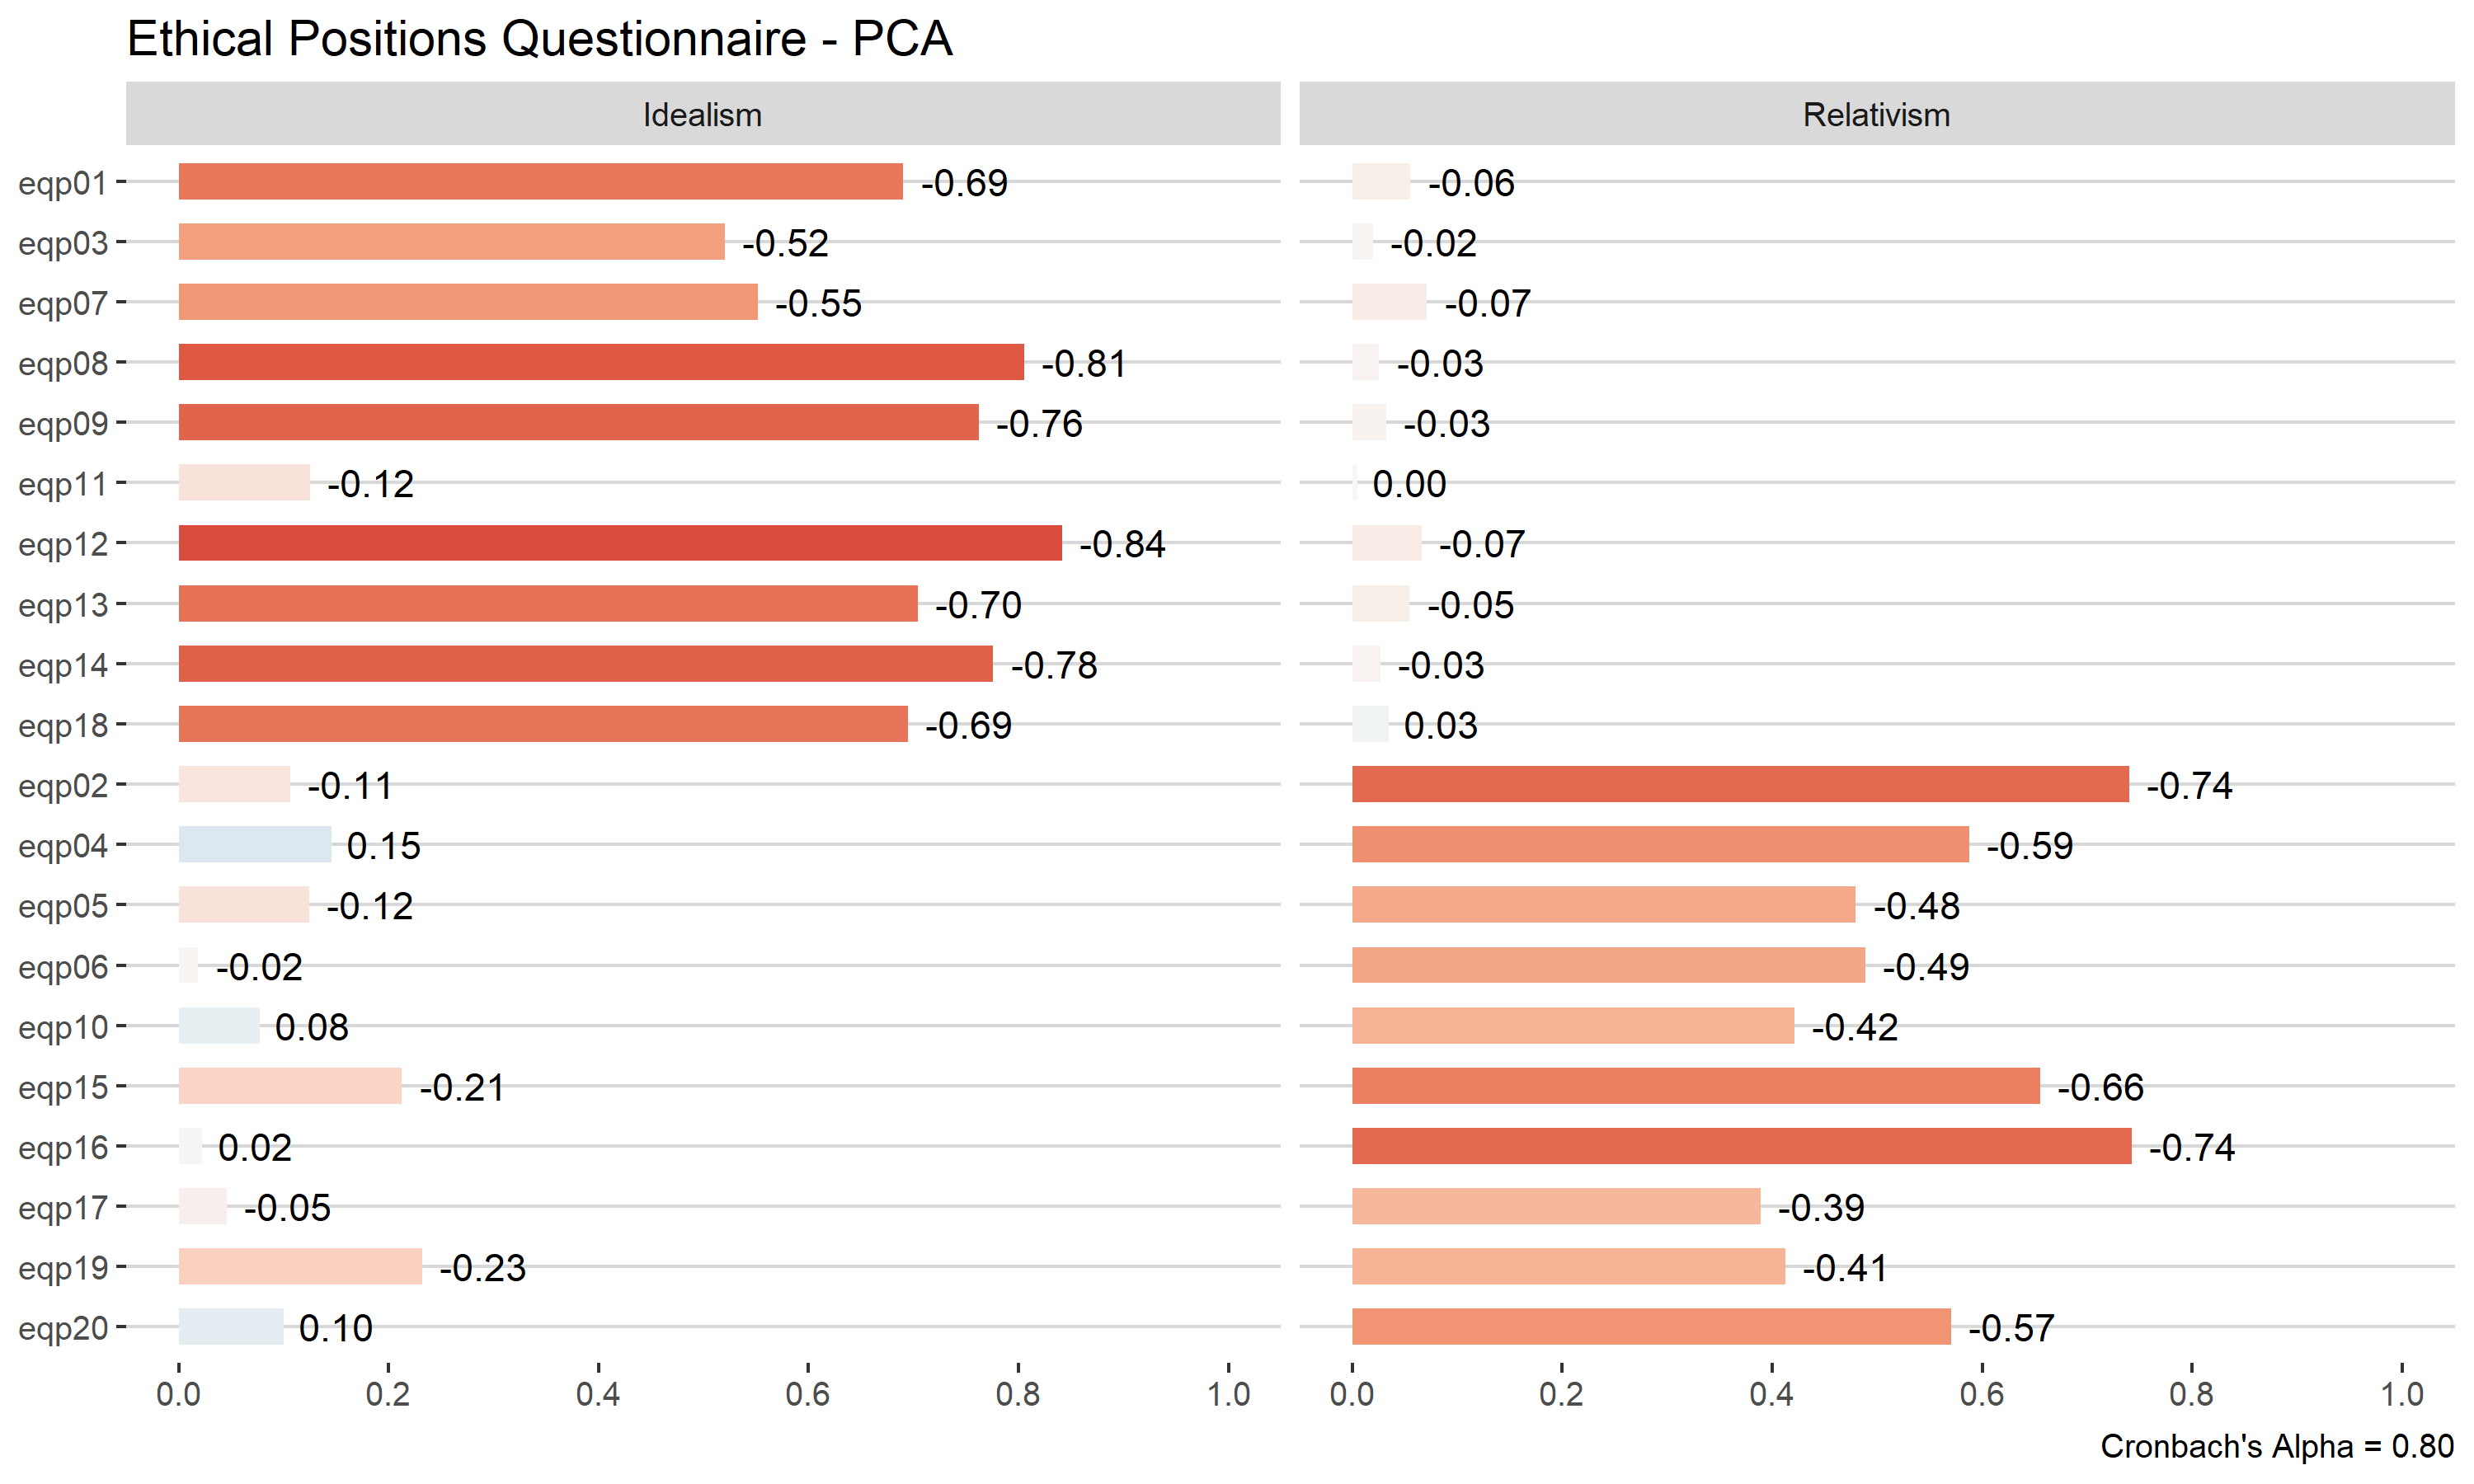
\includegraphics[width=\textwidth]{images/factor_analysis}
    \flushright
{\scriptsize N = 278. Own calculations based on data from Online-Survey Experiment.\par}
\end{figure}

The factor analysis (Figure 1) shows that the variables of the ethical
positions questionaire load very well without any cross-loads (cut off
value: 0.40). Only the loading of eqp11 is too low (-0.12) to take into
account. With the remaining variables the variables Idealism and
Relativism were created.

\hypertarget{randomization-and-descriptive-statistics}{%
\subsection{Randomization and Descriptive
Statistics}\label{randomization-and-descriptive-statistics}}

This section will introduce some basic descriptive statistics of the
used variables. Table 1 shows summary statistics for the used variables.

\begin{table}[ht]
\caption{Summary Statistics}
\centering
\begin{tabular}{rrrrrrrrr}
  \hline
 & N & Mean & SD & Median & Min & Max & Skew & Kurt \\ 
  \hline
Switch Track T1 & 290 & 5.76 & 2.91 & 6 & 1 & 11 & -0.03 & -0.90 \\ 
  Switch Track T2 & 290 & 5.56 & 2.91 & 6 & 1 & 11 & 0.01 & -0.94 \\ 
  Push Person T1 & 290 & 4.29 & 2.83 & 4 & 1 & 11 & 0.55 & -0.72 \\ 
  Push Person T2 & 290 & 4.18 & 2.86 & 4 & 1 & 11 & 0.60 & -0.64 \\ 
  Idealism & 290 & 0 & 1 & 0.18 & -3.40 & 1.73 & -0.86 & 0.37 \\ 
  Relativism & 290 & 0 & 1 & 0.11 & -3.21 & 2.34 & -0.35 & 0.02 \\ 
  Gender & 290 & 1.46 & 0.50 & 1 & 1 & 2 & 0.17 & -1.98 \\ 
  Age & 289 & 24.09 & 3.86 & 23 & 18 & 53 & 2.14 & 10.52 \\ 
  Church Attendance & 278 & 1.87 & 1.04 & 2 & 1 & 6 & 1.38 & 2.06 \\ 
  Control Group & 290 & 0.32 & 0.47 & 0 & 0 & 1 & 0.78 & -1.39 \\ 
  Discussion Group & 290 & 0.34 & 0.47 & 0 & 0 & 1 & 0.67 & -1.56 \\ 
  Information Group & 290 & 0.34 & 0.47 & 0 & 0 & 1 & 0.67 & -1.56 \\ 
   \hline
\end{tabular}
\end{table}

Figure 2 shows a comparison between the experimental groups by age,
gender, Idealism and Relativism. As mentioned before, the randomization
of the groups was flawed. Regarding the comparison between the
experimental groups by age and gender, the differences are significant.
The control group has a women proportion of over 52\%, whereas only 41\%
of the discussion group are women. In addition, there is a strong
outlier in the control group with over 50 years in the age.

\begin{figure}
    \caption{Randomization - Sociodemographics}
    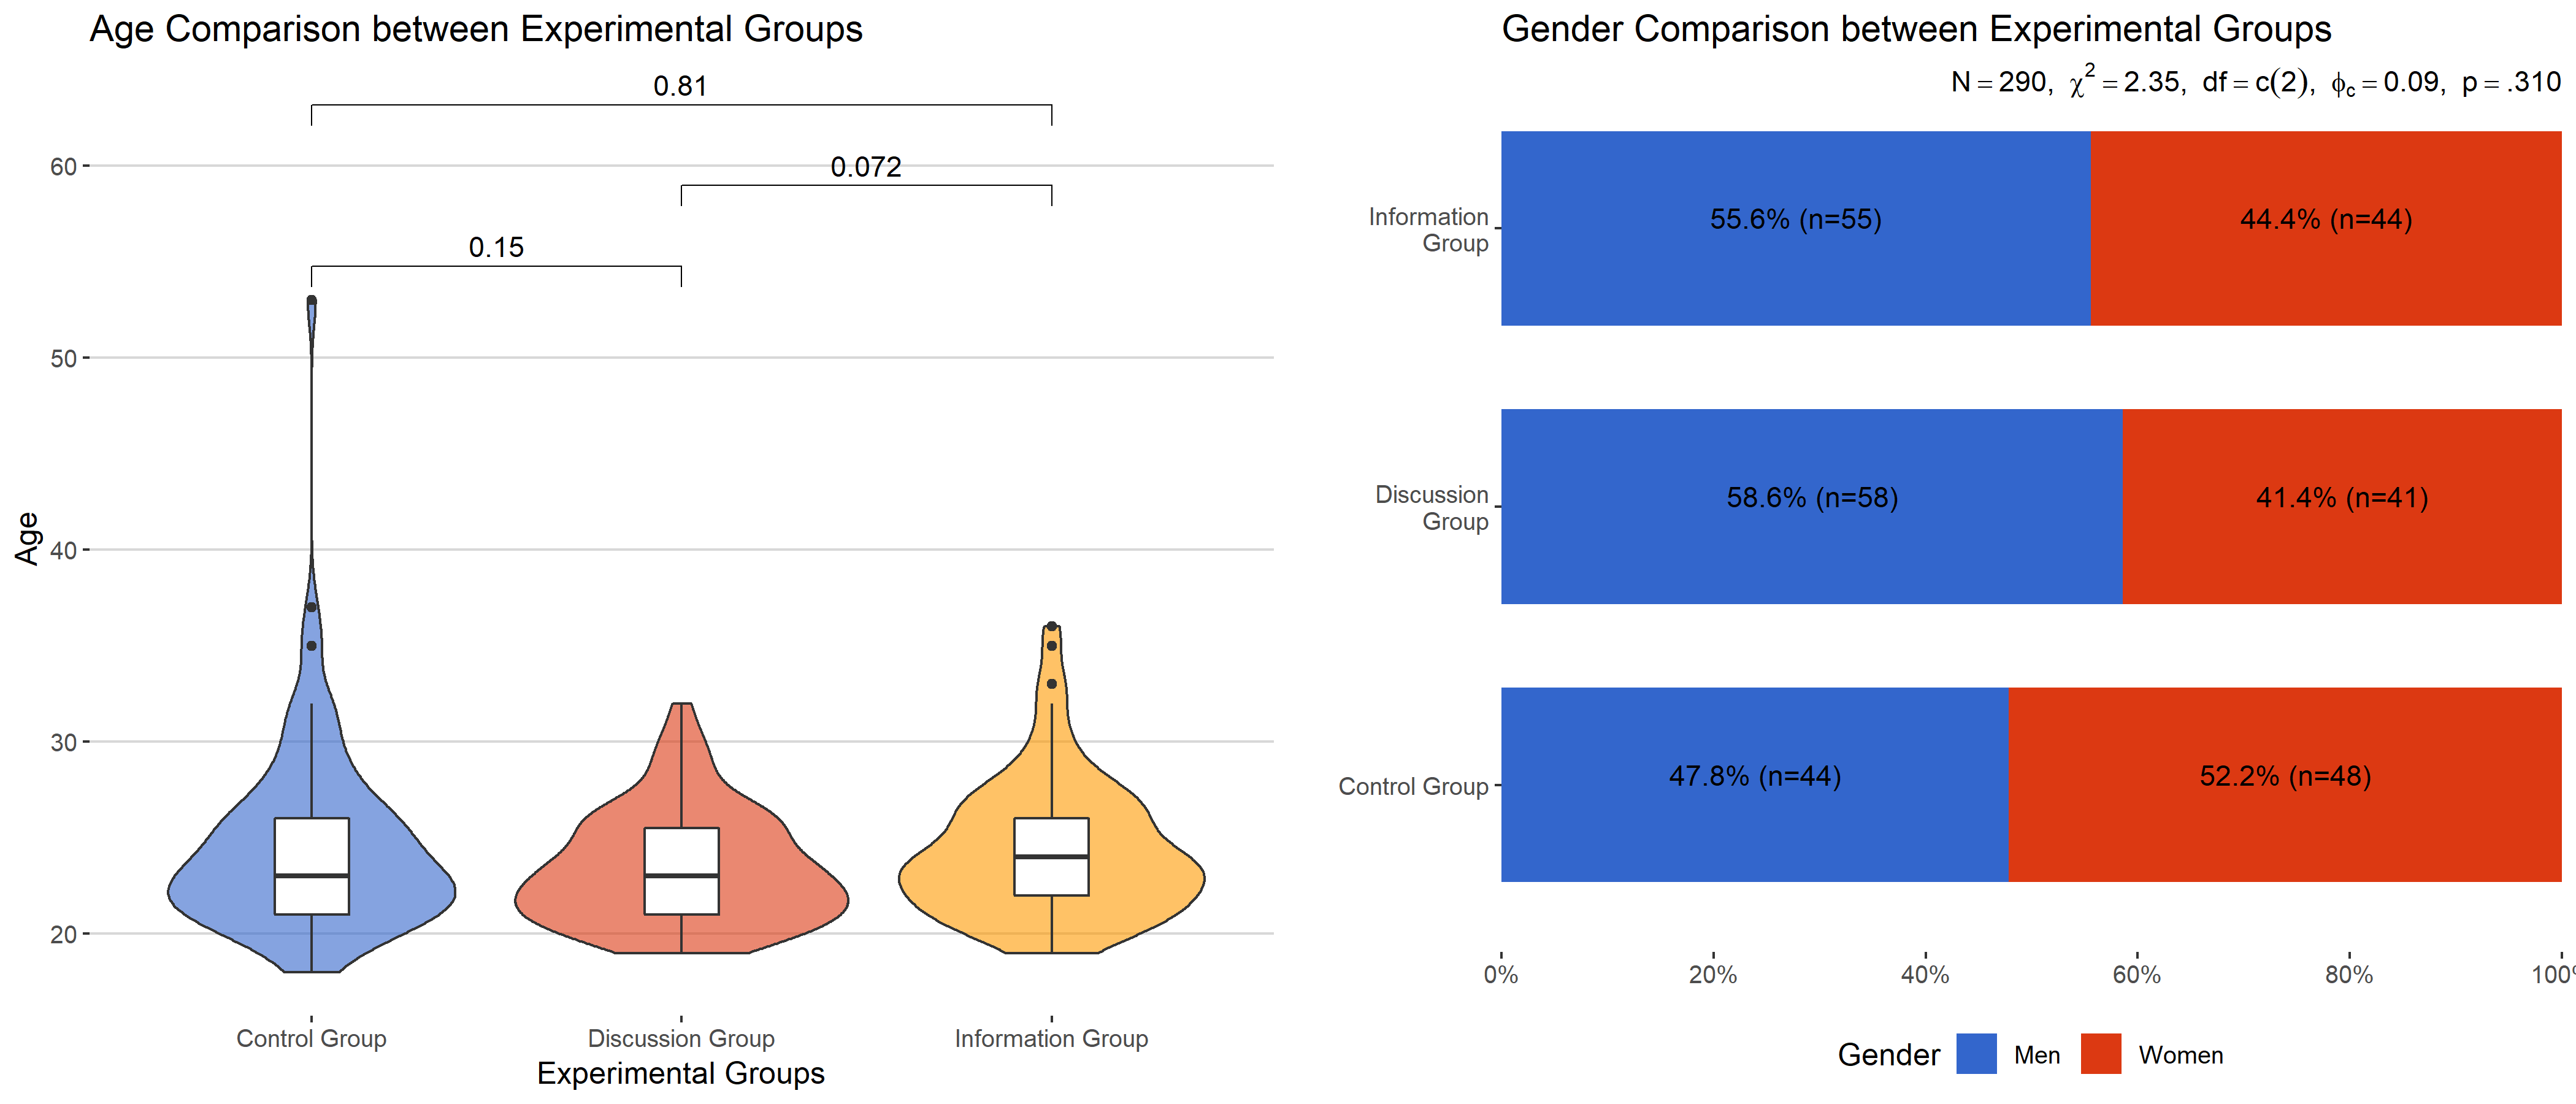
\includegraphics[width=\textwidth]{images/dem_compare}
    \flushright
{\scriptsize N = 278. P-Values are reported. Own calculations based on data from Online-Survey Experiment.\par}
\end{figure}

Moreover, there are also significant differences between the
experimental groups regarding the main independent variables Idealism
and Relativism. Concerning this issue, the following analysis should be
interpreted with caution.

When it comes to the question of whether it is morally justifiable to
switch the track or even push a person, there are differences in age and
gender (see Figure 3).

\begin{figure}[!h]
    \caption{Randomization - Dependent Variables}
    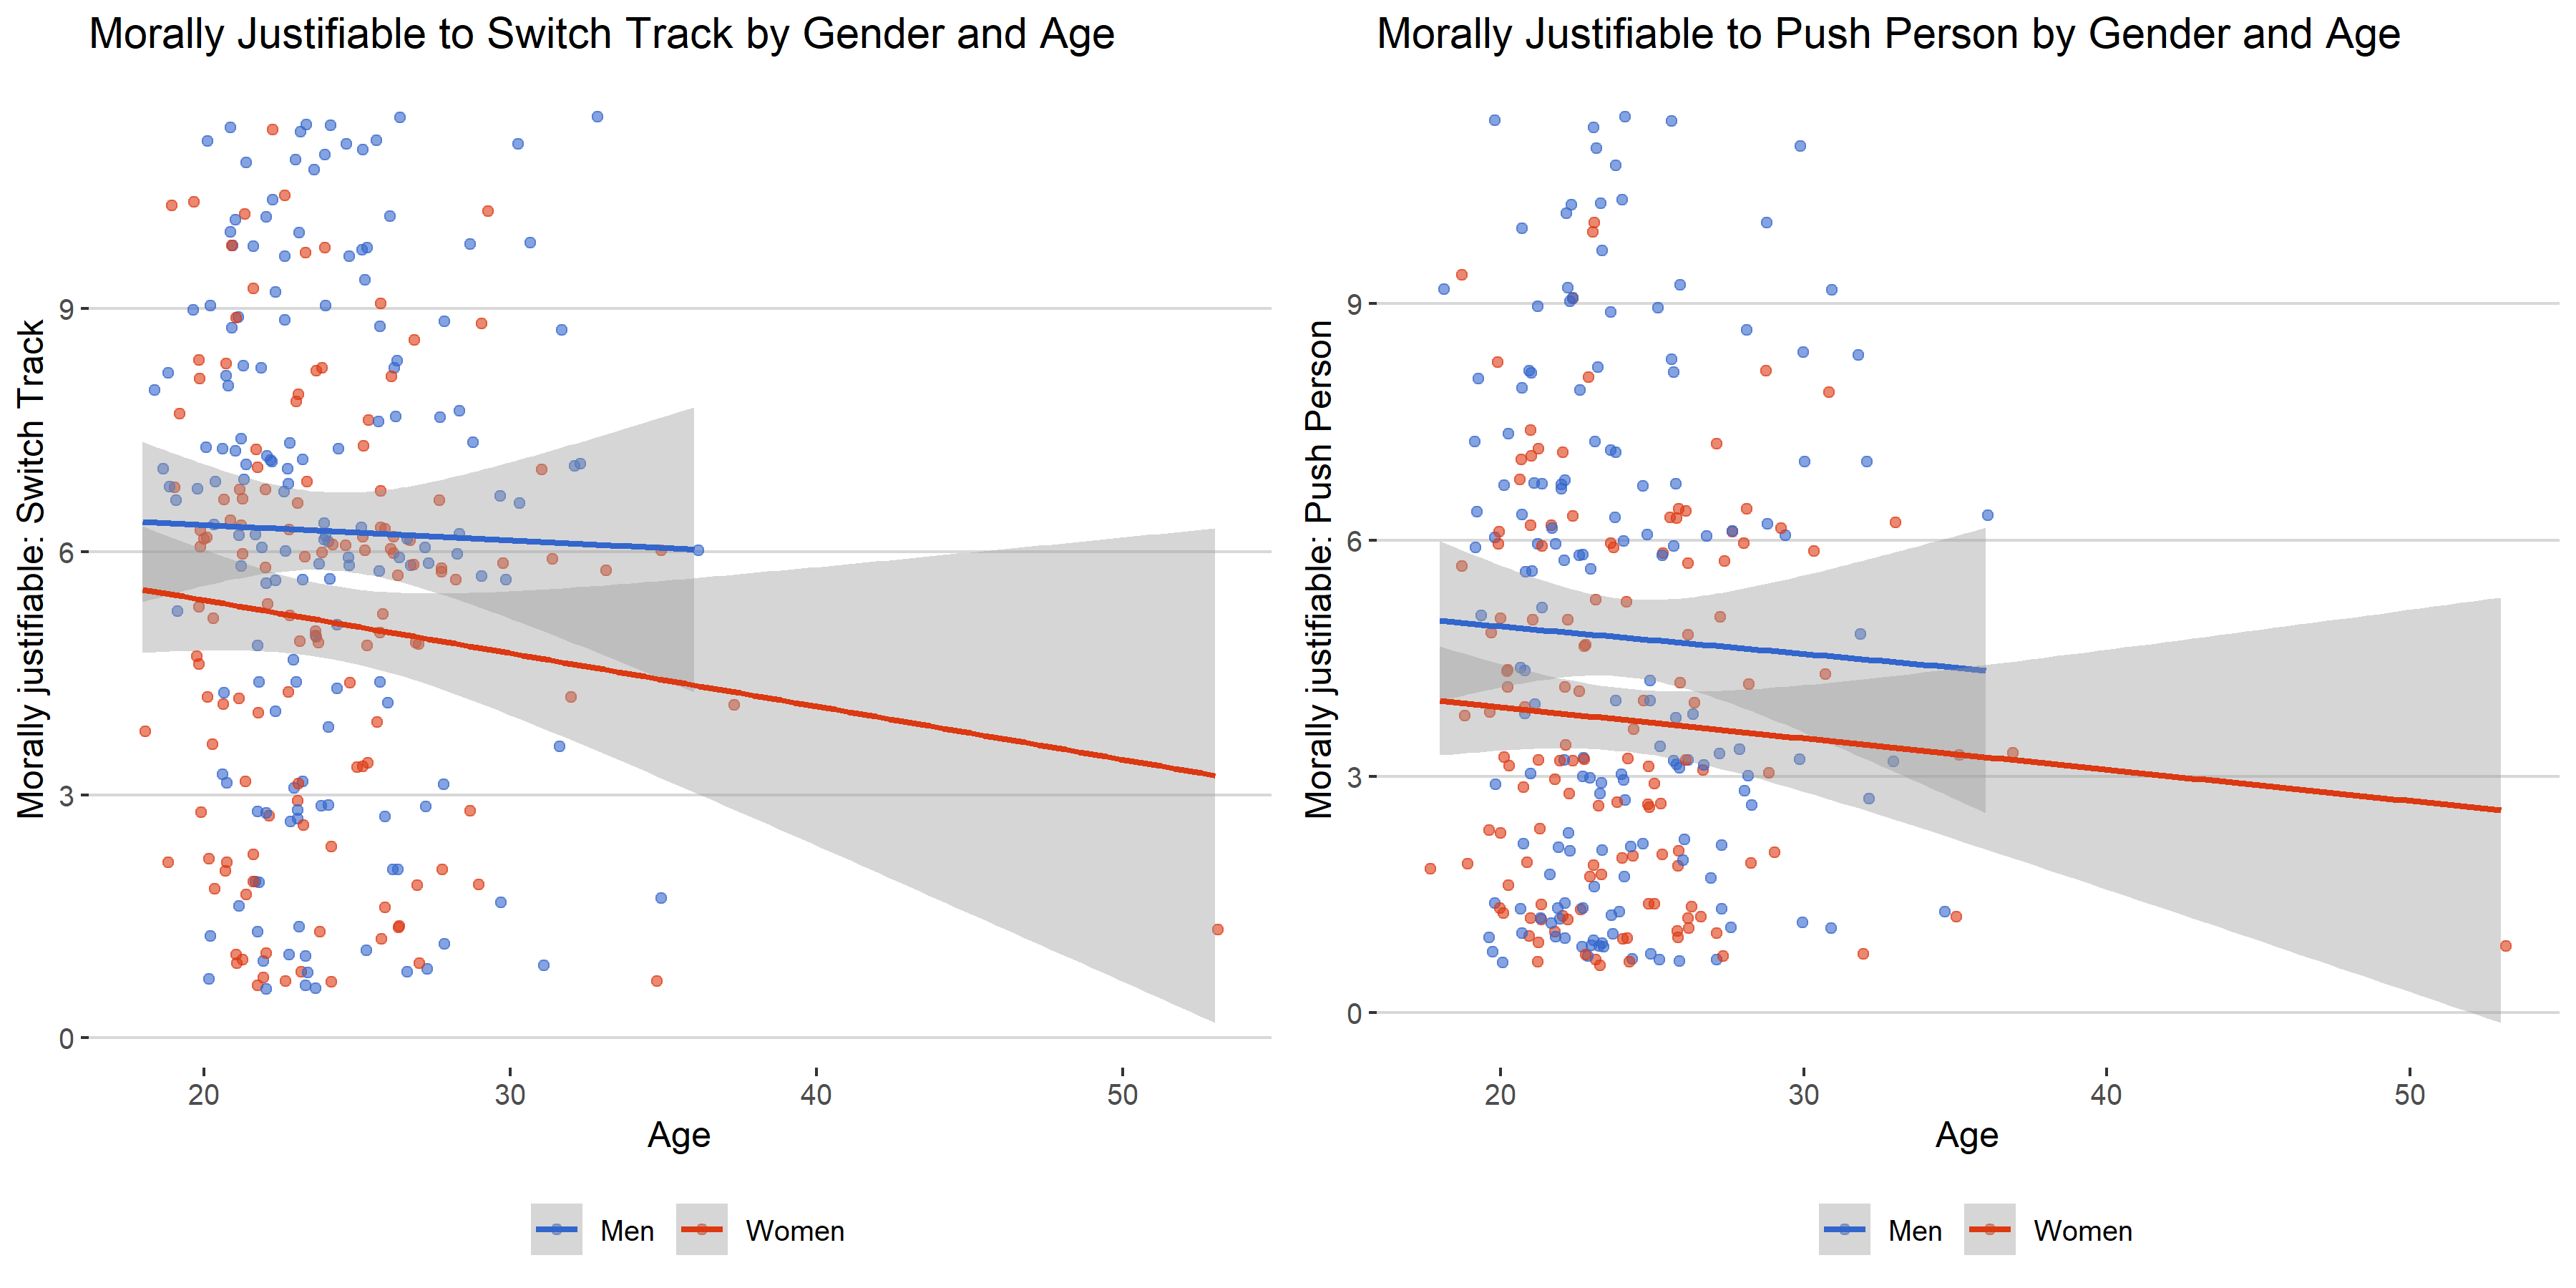
\includegraphics[width=\textwidth]{images/gender_av_compare}
    \flushright
{\scriptsize N = 278. Own calculations based on data from Online-Survey Experiment.\par}
\end{figure}

Older people as well as female persons consider both scenarios less
morally justified. A comparison of the means, regarding the gender, the
differences between men and women are clearly significant in both
scenarios. However, comparing the two scenarios shows that switching
tracks is more likely to be morally justified than pushing a person.

\begin{figure}[!h]
    \caption{Randomization - Independent Variables}
    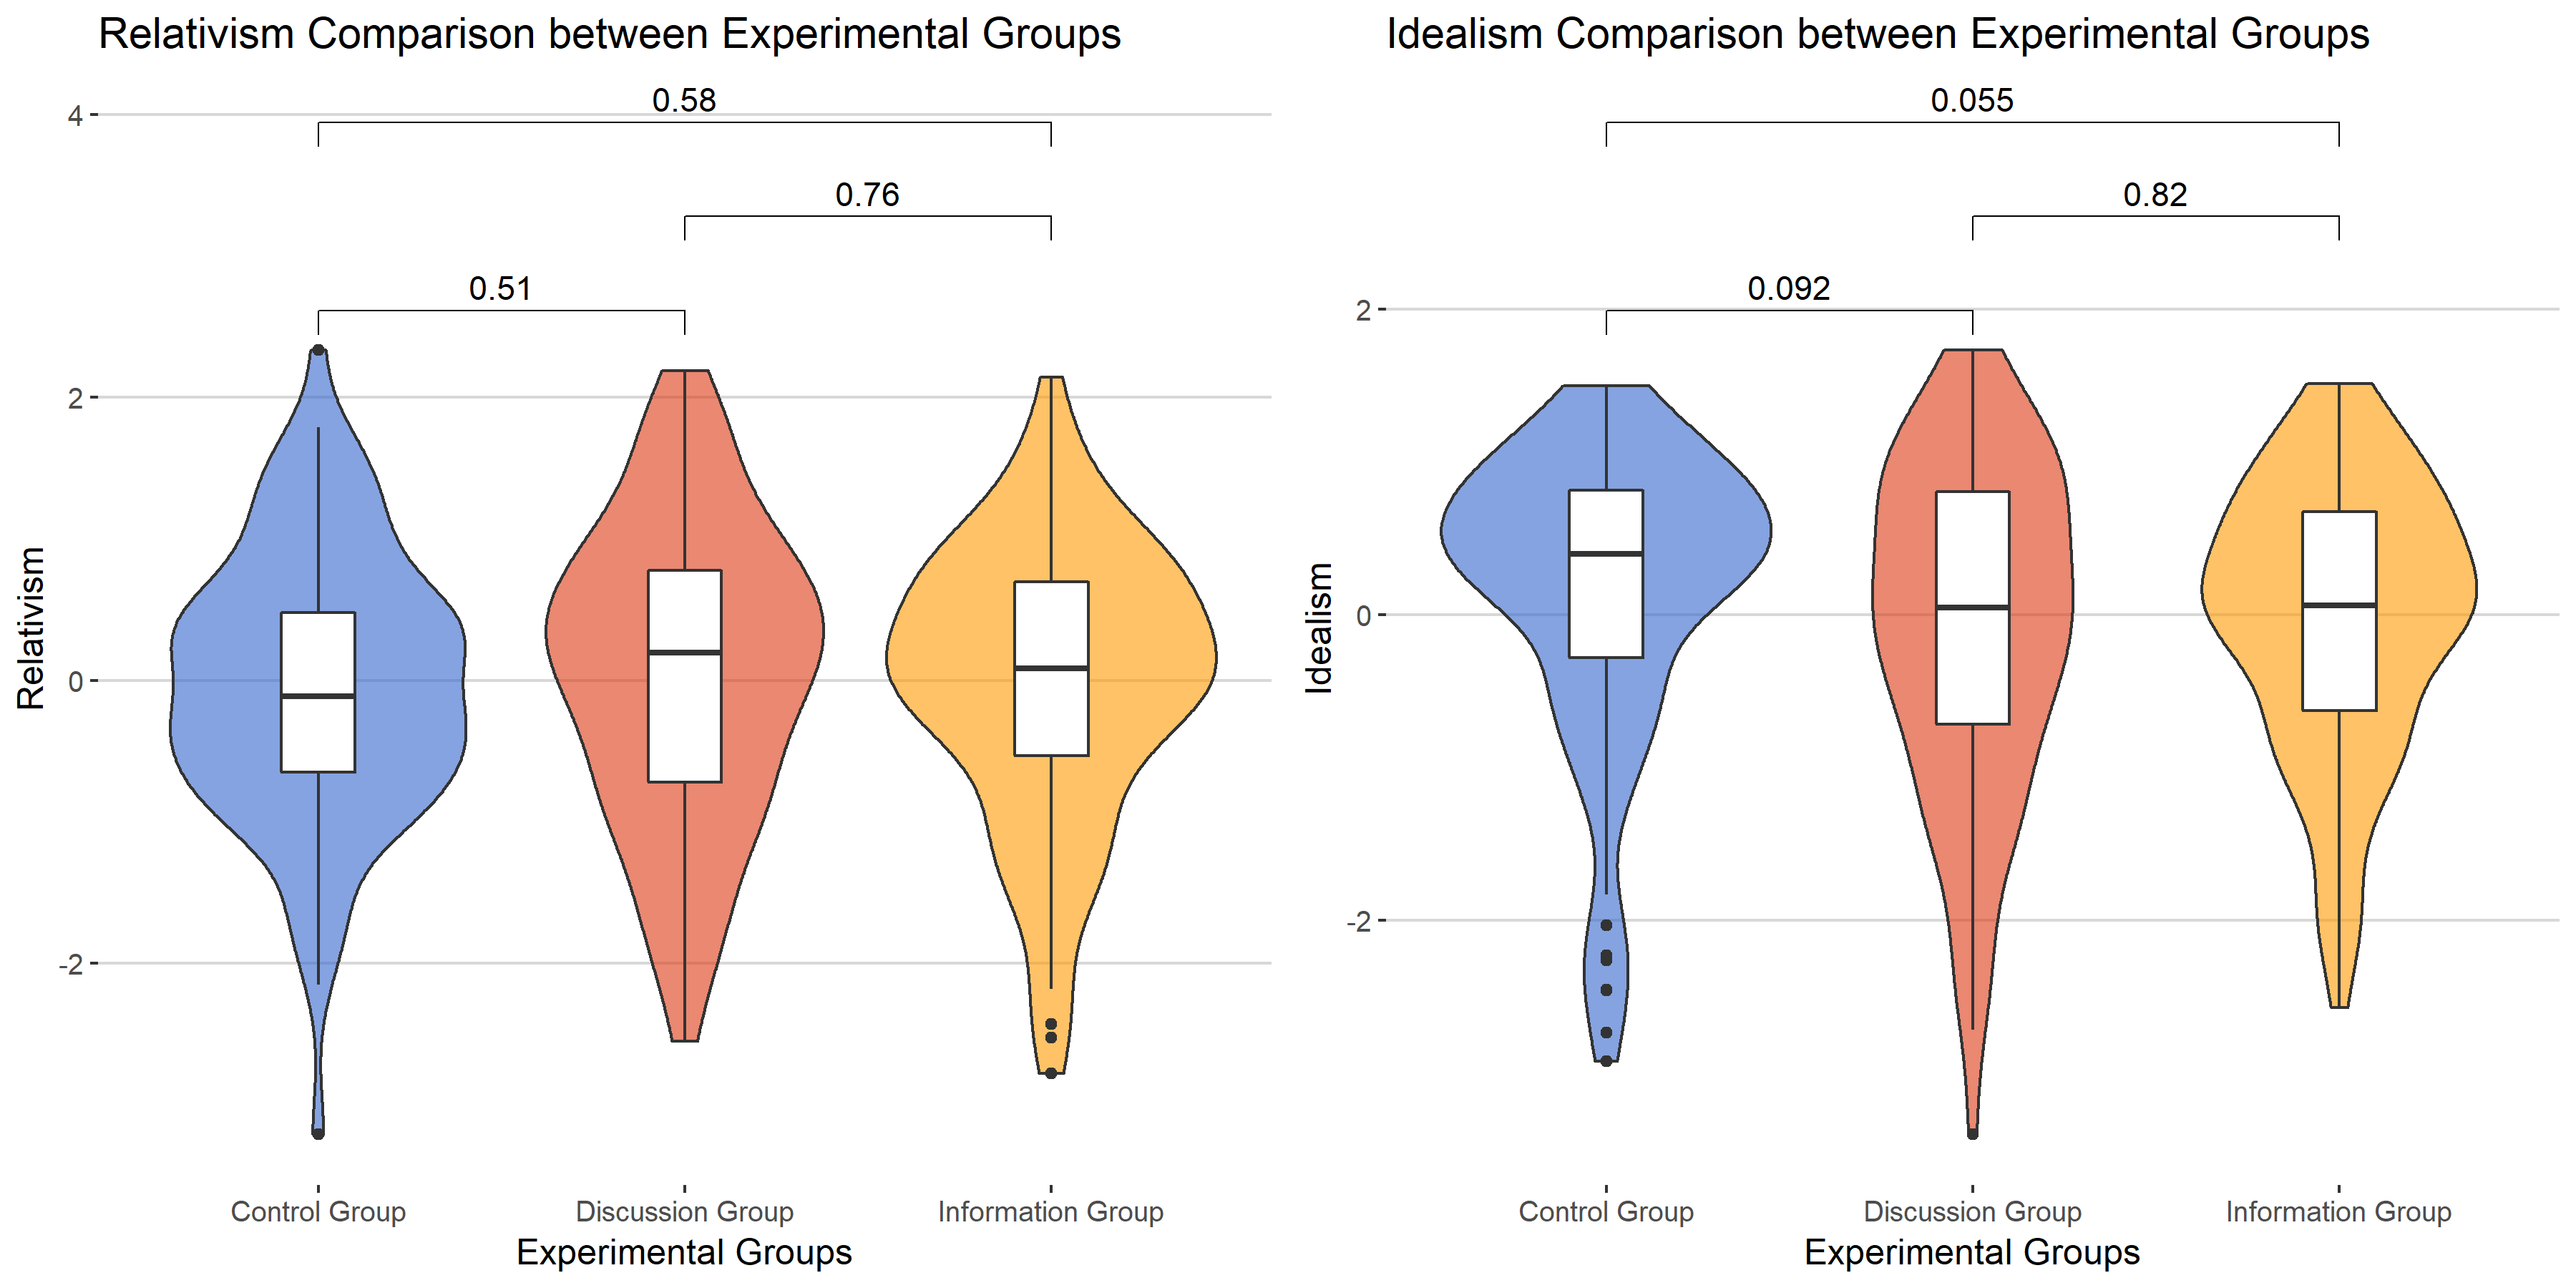
\includegraphics[width=\textwidth]{images/uv_compare}
    \flushright
{\scriptsize N = 278. P-Values are reported. Own calculations based on data from Online-Survey Experiment.\par}
\end{figure}

\newpage
\section{Analysis} \label{analysis}

In this Section, the regression models are reported and interpreted in
regard to their implications for the previously derived hypotheses. In
sum, XX models were estimated, which are depicted in coefficient plots
(see plot XX to XX).

\begin{figure}[!h]
    \caption{Models 1}
    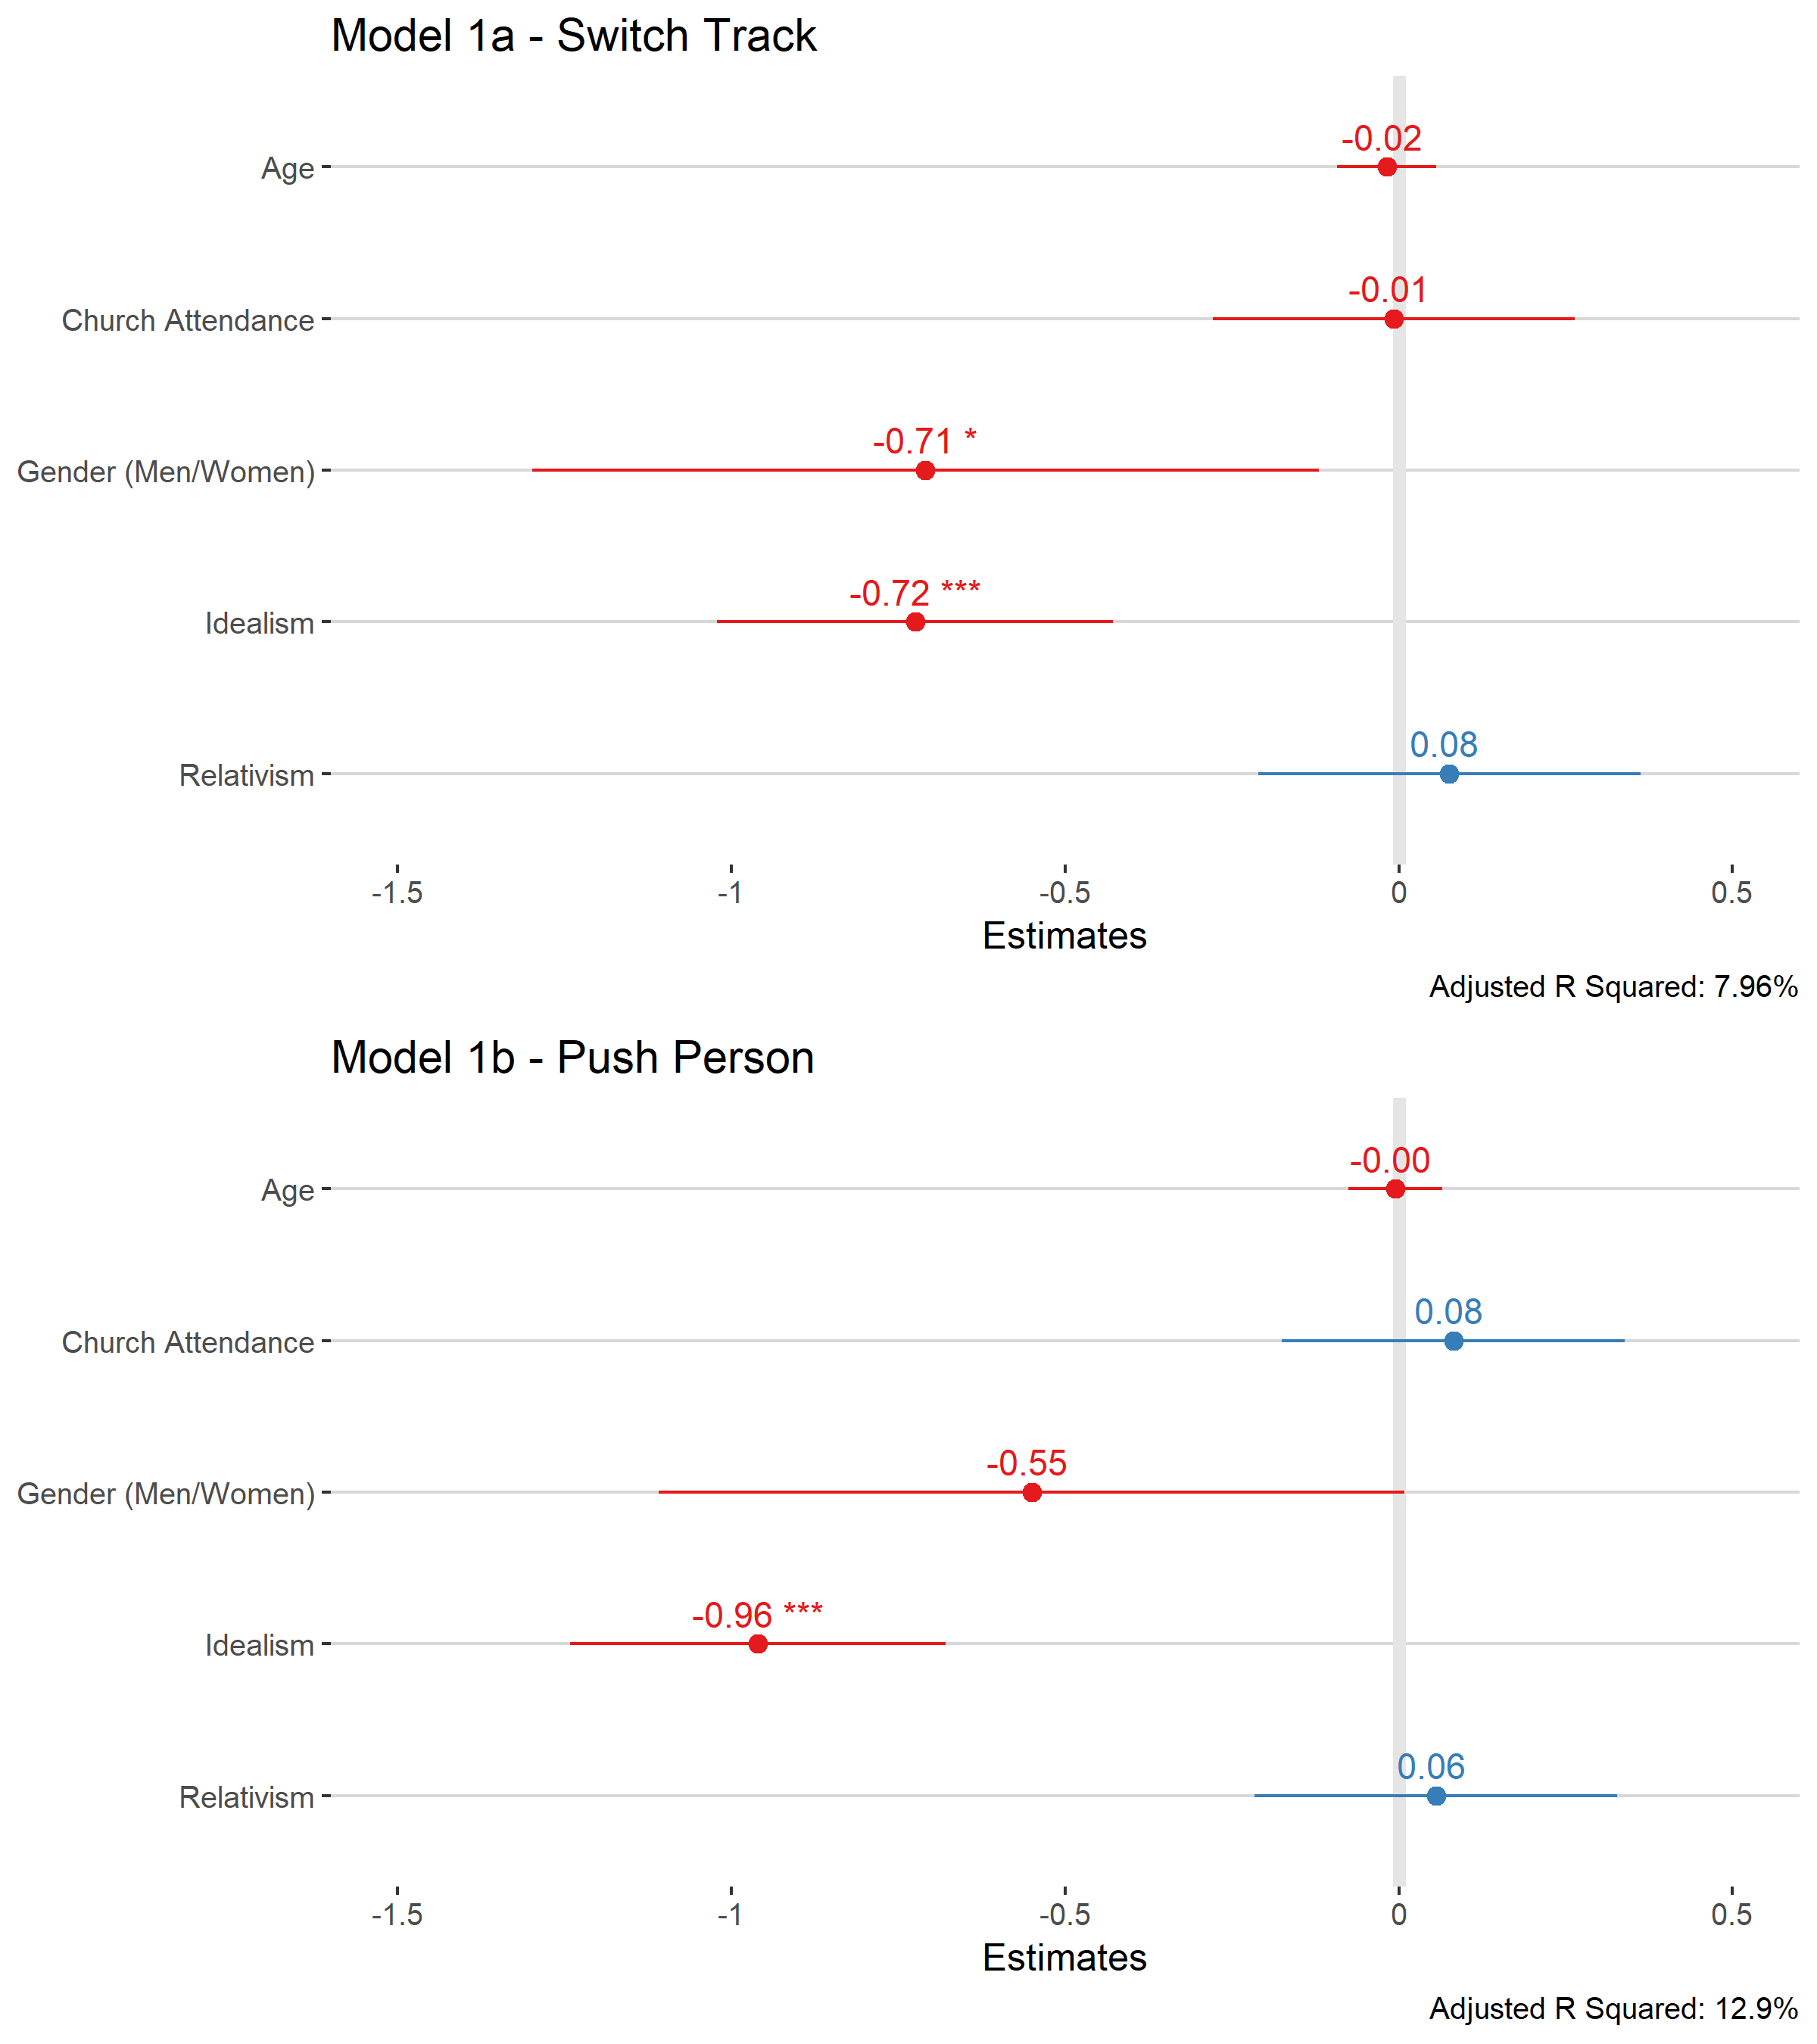
\includegraphics[width=\textwidth]{images/reg1_combined}
    \flushright
{\scriptsize $^{***}p<0.001$, $^{**}p<0.01$, $^*p<0.05$.  Unstandardized regression coefficients. 90\% confidence intervals are shown. \\ Own calculations based on data from Online-Survey Experiment.\par}
\end{figure}

First, the models with the dependent variable at time t1 (before the
treatment) are analyzed. Model 1a shows the results for scenario 1,
model 1b for scenario 2. The factor idealism has a strong negative
effect, meaning that the more idealistic a person is, the less they tend
to switch and push (Model 1a: b = xx , p\textless{} 0.001 and Model 1b:
b = xx , p\textless{} 0.001) . Relativism in turn has a positive sign,
but is statistically insignificant and has only a marginal coefficient
size (Model 1a: b = and Model 1b: b = ). It has to be noted that the
R\^{}2 statistics are not particularly large, indicating only 9, 6\% and
14,5\% explained variance of the dependent variable for the Models 1a
and 1b, respectively. Nevertheless, for the previously derived
hypotheses H1a, which states that, the more idealist an individual, the
less likely it will switch/push, confirming evidence can be noted. The
same holds true for H1b, which assumes that relativism has no effect on
an individual's decision to switch/push.

\begin{figure}[!h]
    \caption{Models 2 - Idealism}
    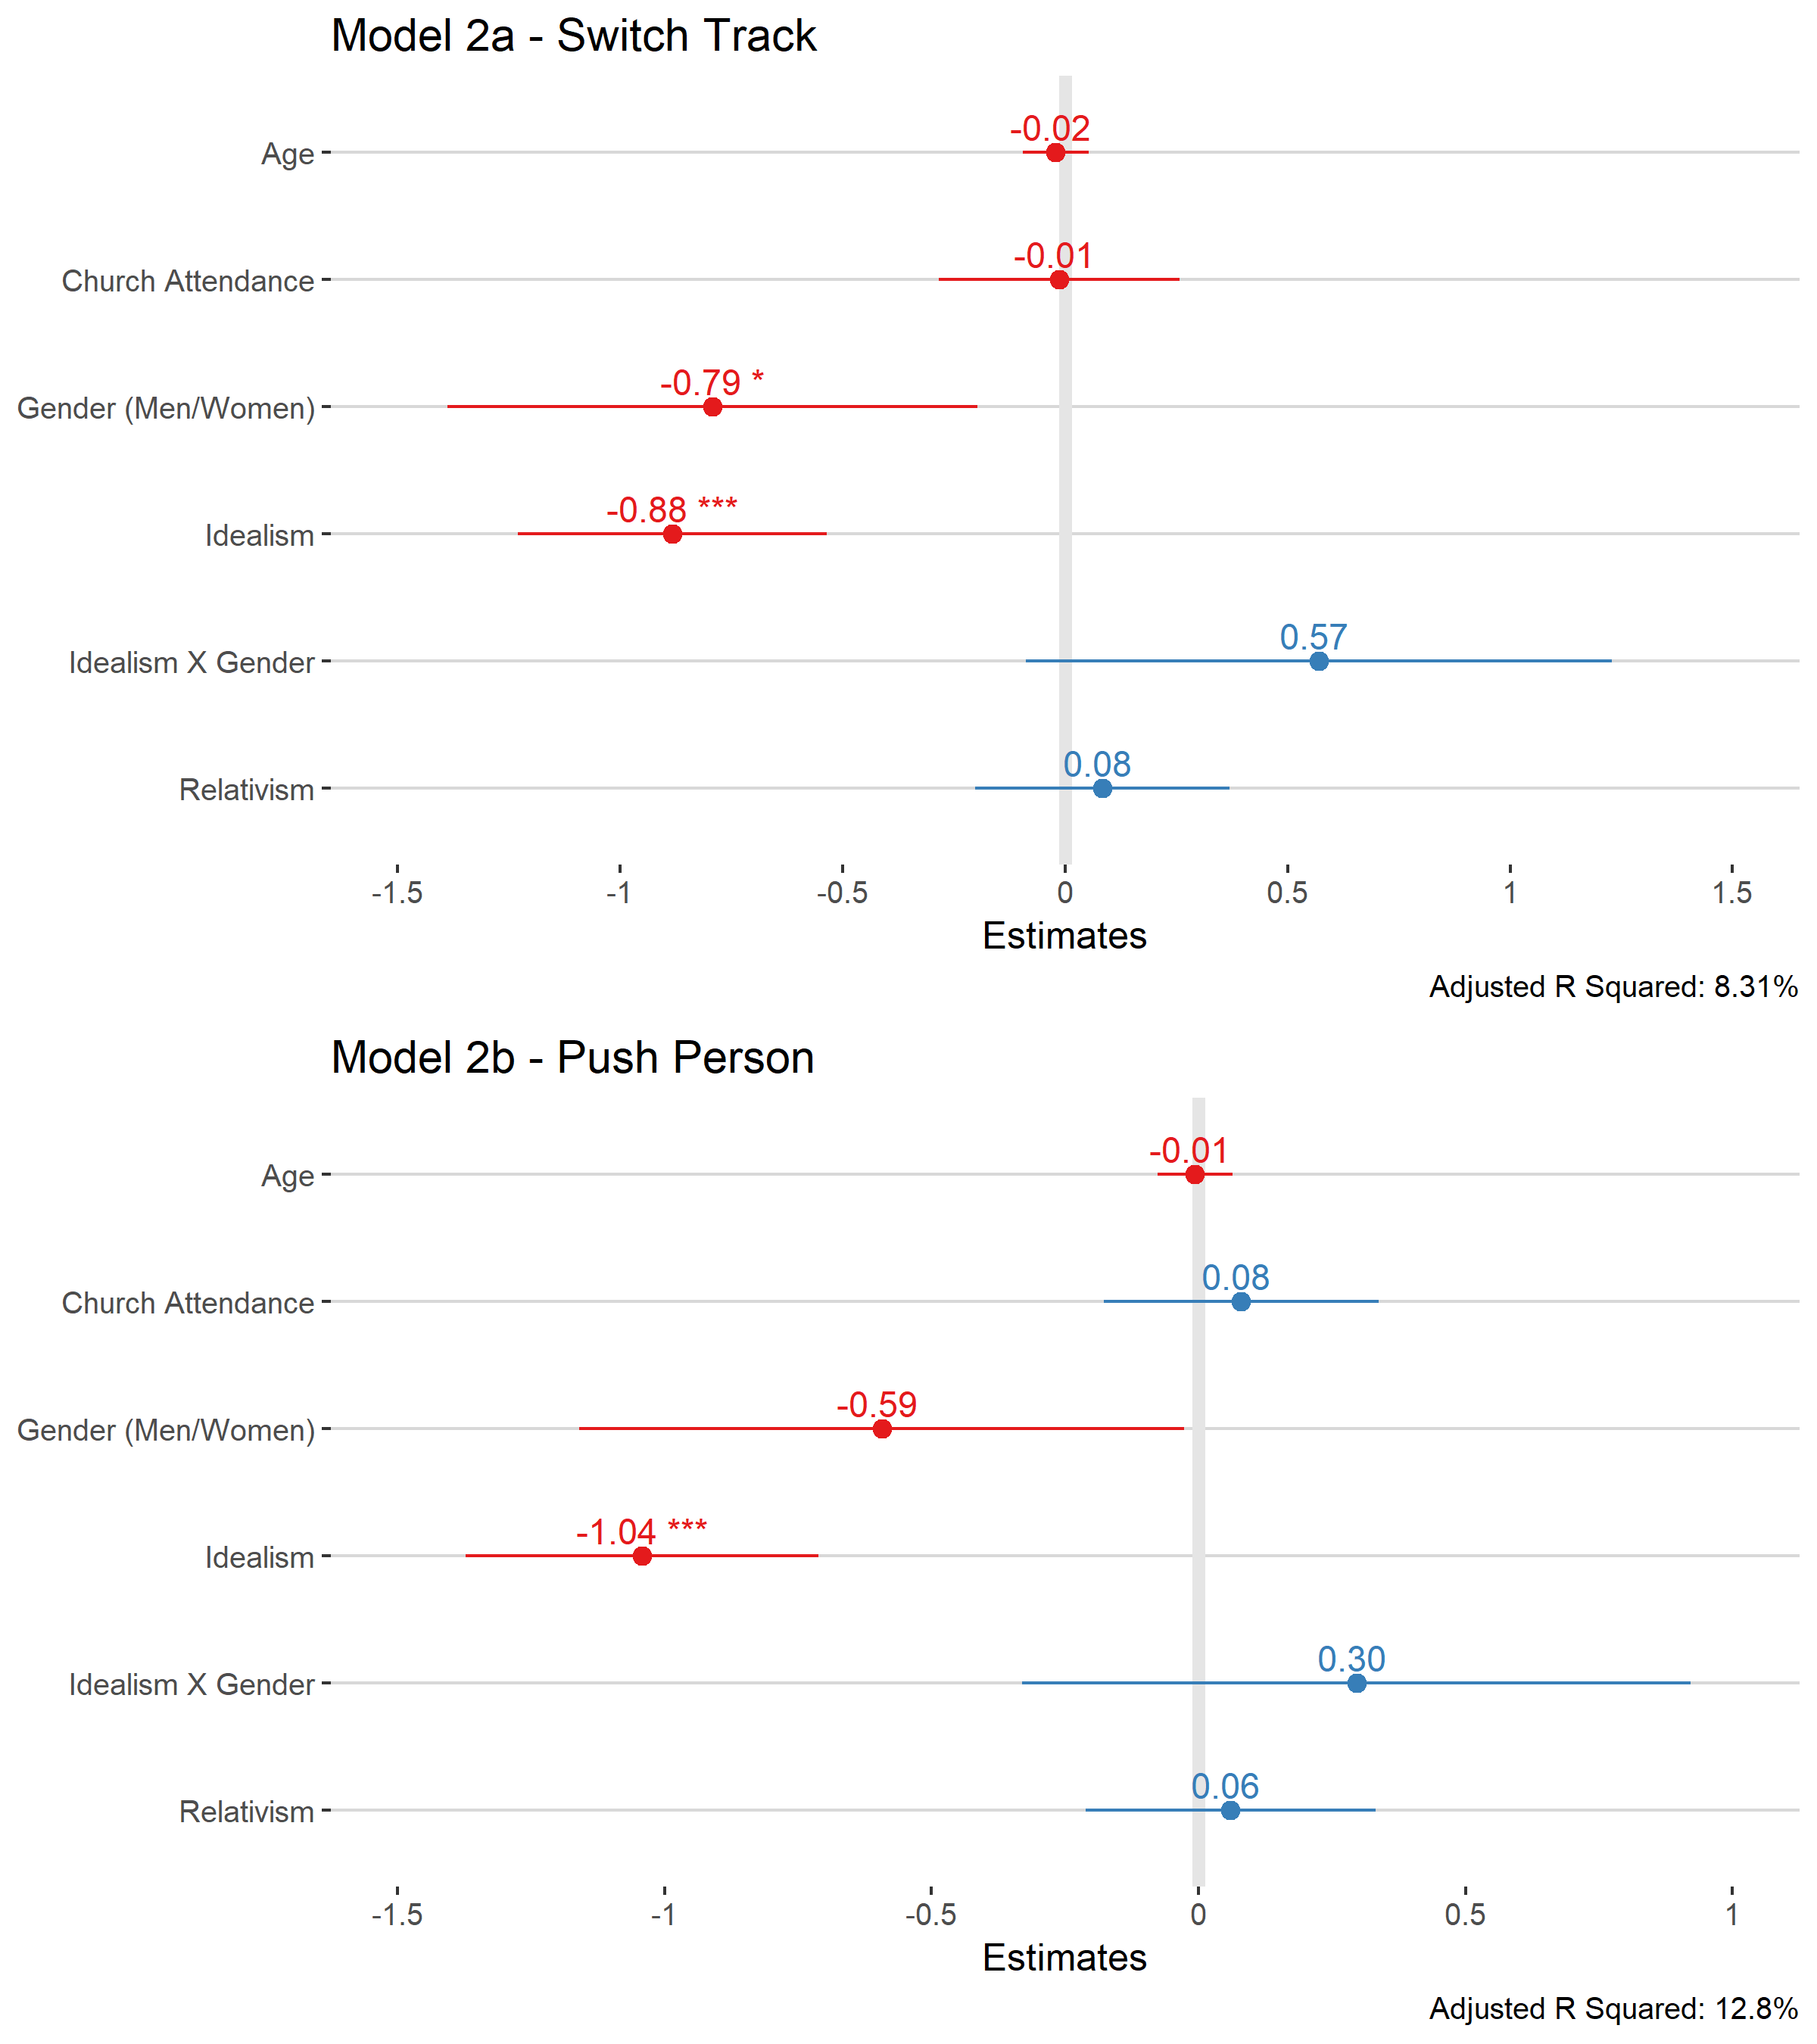
\includegraphics[width=\textwidth]{images/reg2_c1_idealism}
    \flushright
{\scriptsize $^{***}p<0.001$, $^{**}p<0.01$, $^*p<0.05$.  N = 278. Unstandardized regression coefficients. 90\% confidence intervals are shown. \\ Own calculations based on data from Online-Survey Experiment.\par}
\end{figure}

As a next step, models with the dependent variable after the treatment
are estimated (t2). Here, we control for the variable at the time t1,
which means that the other independent variables only predict the
variance of the dependent variable which differs from the one at t1.
Positive coefficients indicate opinion change in the direction of higher
values on the dependent variable, negative coefficients in turn indicate
negative opinion change. In general, the R\^{}2 values in all of the
t2-models therefore indicate a high amount of explained variance, due to
the fact that the judgment at the time t2 is highly dependent on the
judgment at t1, wich is included in the models.

\begin{figure}[!h]
    \caption{Models 2 - Idealism Interaction Plots}
    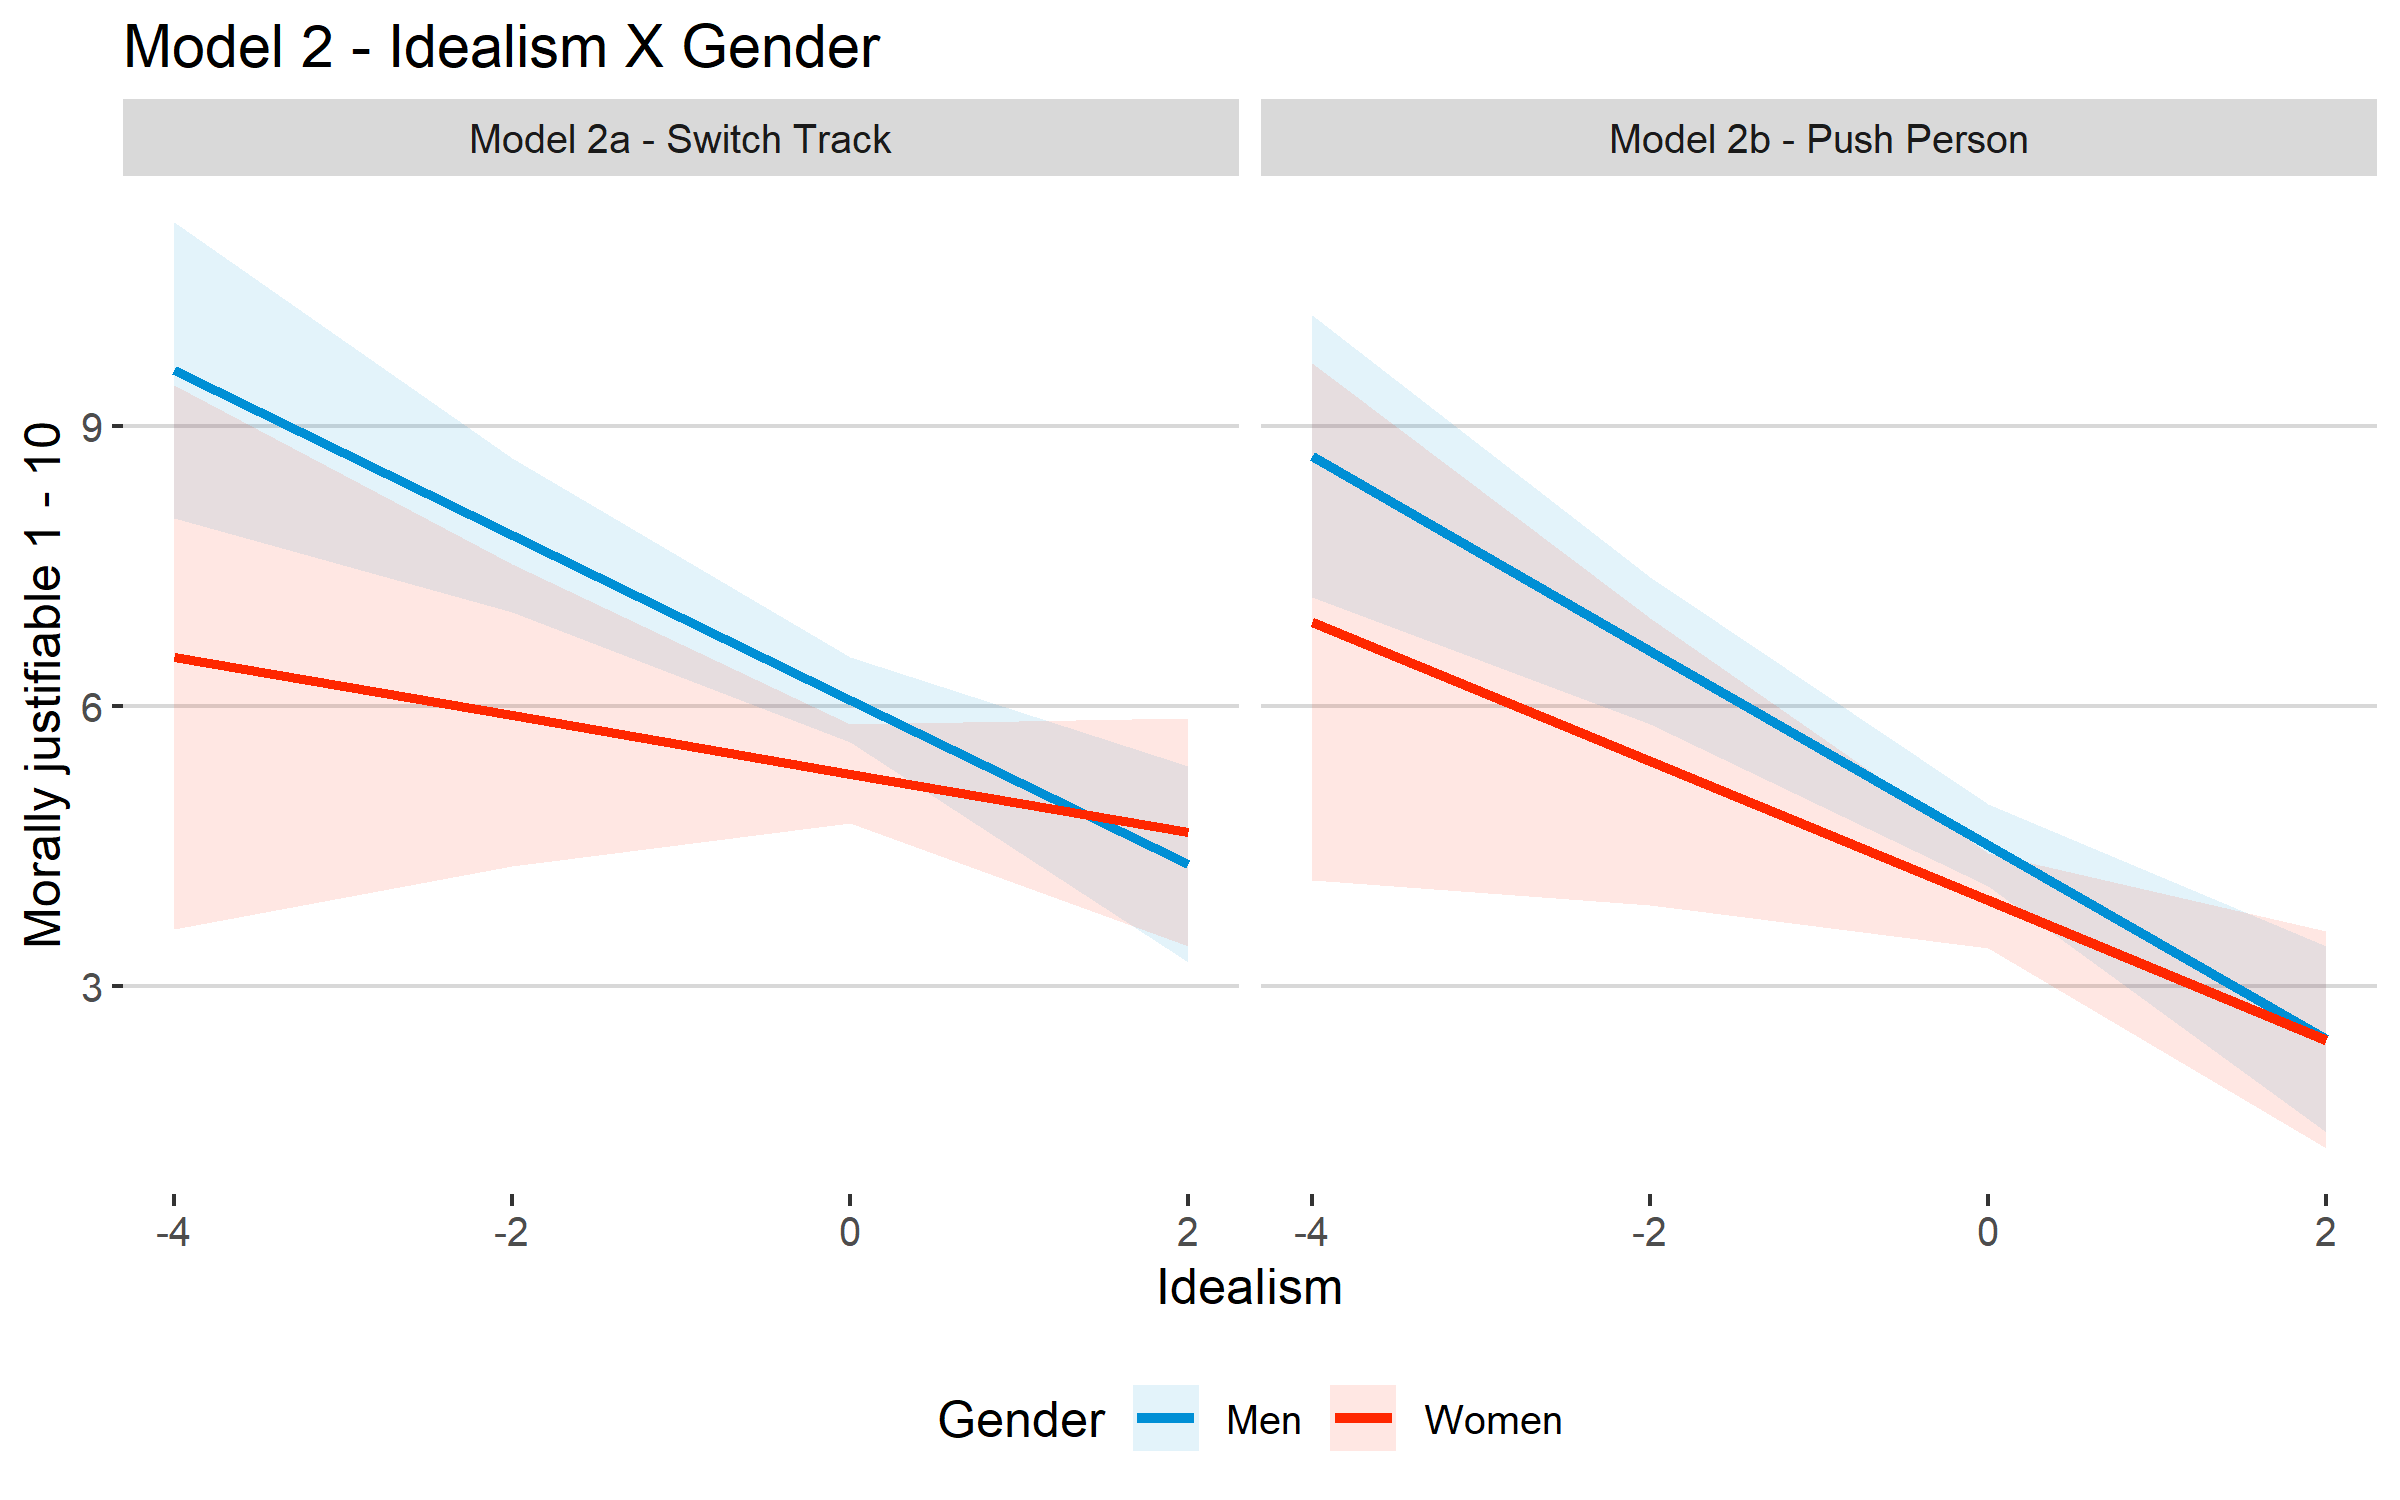
\includegraphics[width=\textwidth]{images/reg2_c2_idealism}
    \flushright
{\scriptsize N = 278. 90\% confidence intervals are shown. \\ Own calculations based on data from Online-Survey Experiment.\par}
\end{figure}

Model 2a depicts the results for the scenario 1 dependent variable,
Model 2b for scenario 2 (see plot XX and XX). First, it comes to
attention that the treatments have a strong effect. The discussion group
has negative coefficients for both scenarios, indicating that persons
which engaged in discussion had, compared to persons of the control
group, a opinion change in the direction of \enquote{not
switching/pushing} (Model 2a: b = -0.73, p\textless{} 0.01 and Model 2b:
b = -0.81,p\textless{} 0.01). Regarding the information group, these
effects can be observed as well, although not as strong (Model 2a: b =
-0.46, p\textless{} 0.05 and Model 2b: b = -0.56, p\textless{} 0.05).
The opinion change in the discussion group is more negative, but the
differences to the information group are not as large and not
statistically significant. Regarding idealism, for scenario 1 a rather
weak and insignificant effect can be observed (b = -0.15), while
relativism has no observable effect on opinion change at all (b = 0.00).
The results for scenario 2 are insignificant as well, but differ in
regard to relativism, which now has a weak negative effect (b = -0.14),
while the effect of idealism did not change much (b = -0.09).

\begin{figure}[!h]
    \caption{Models 3 - Relativism}
    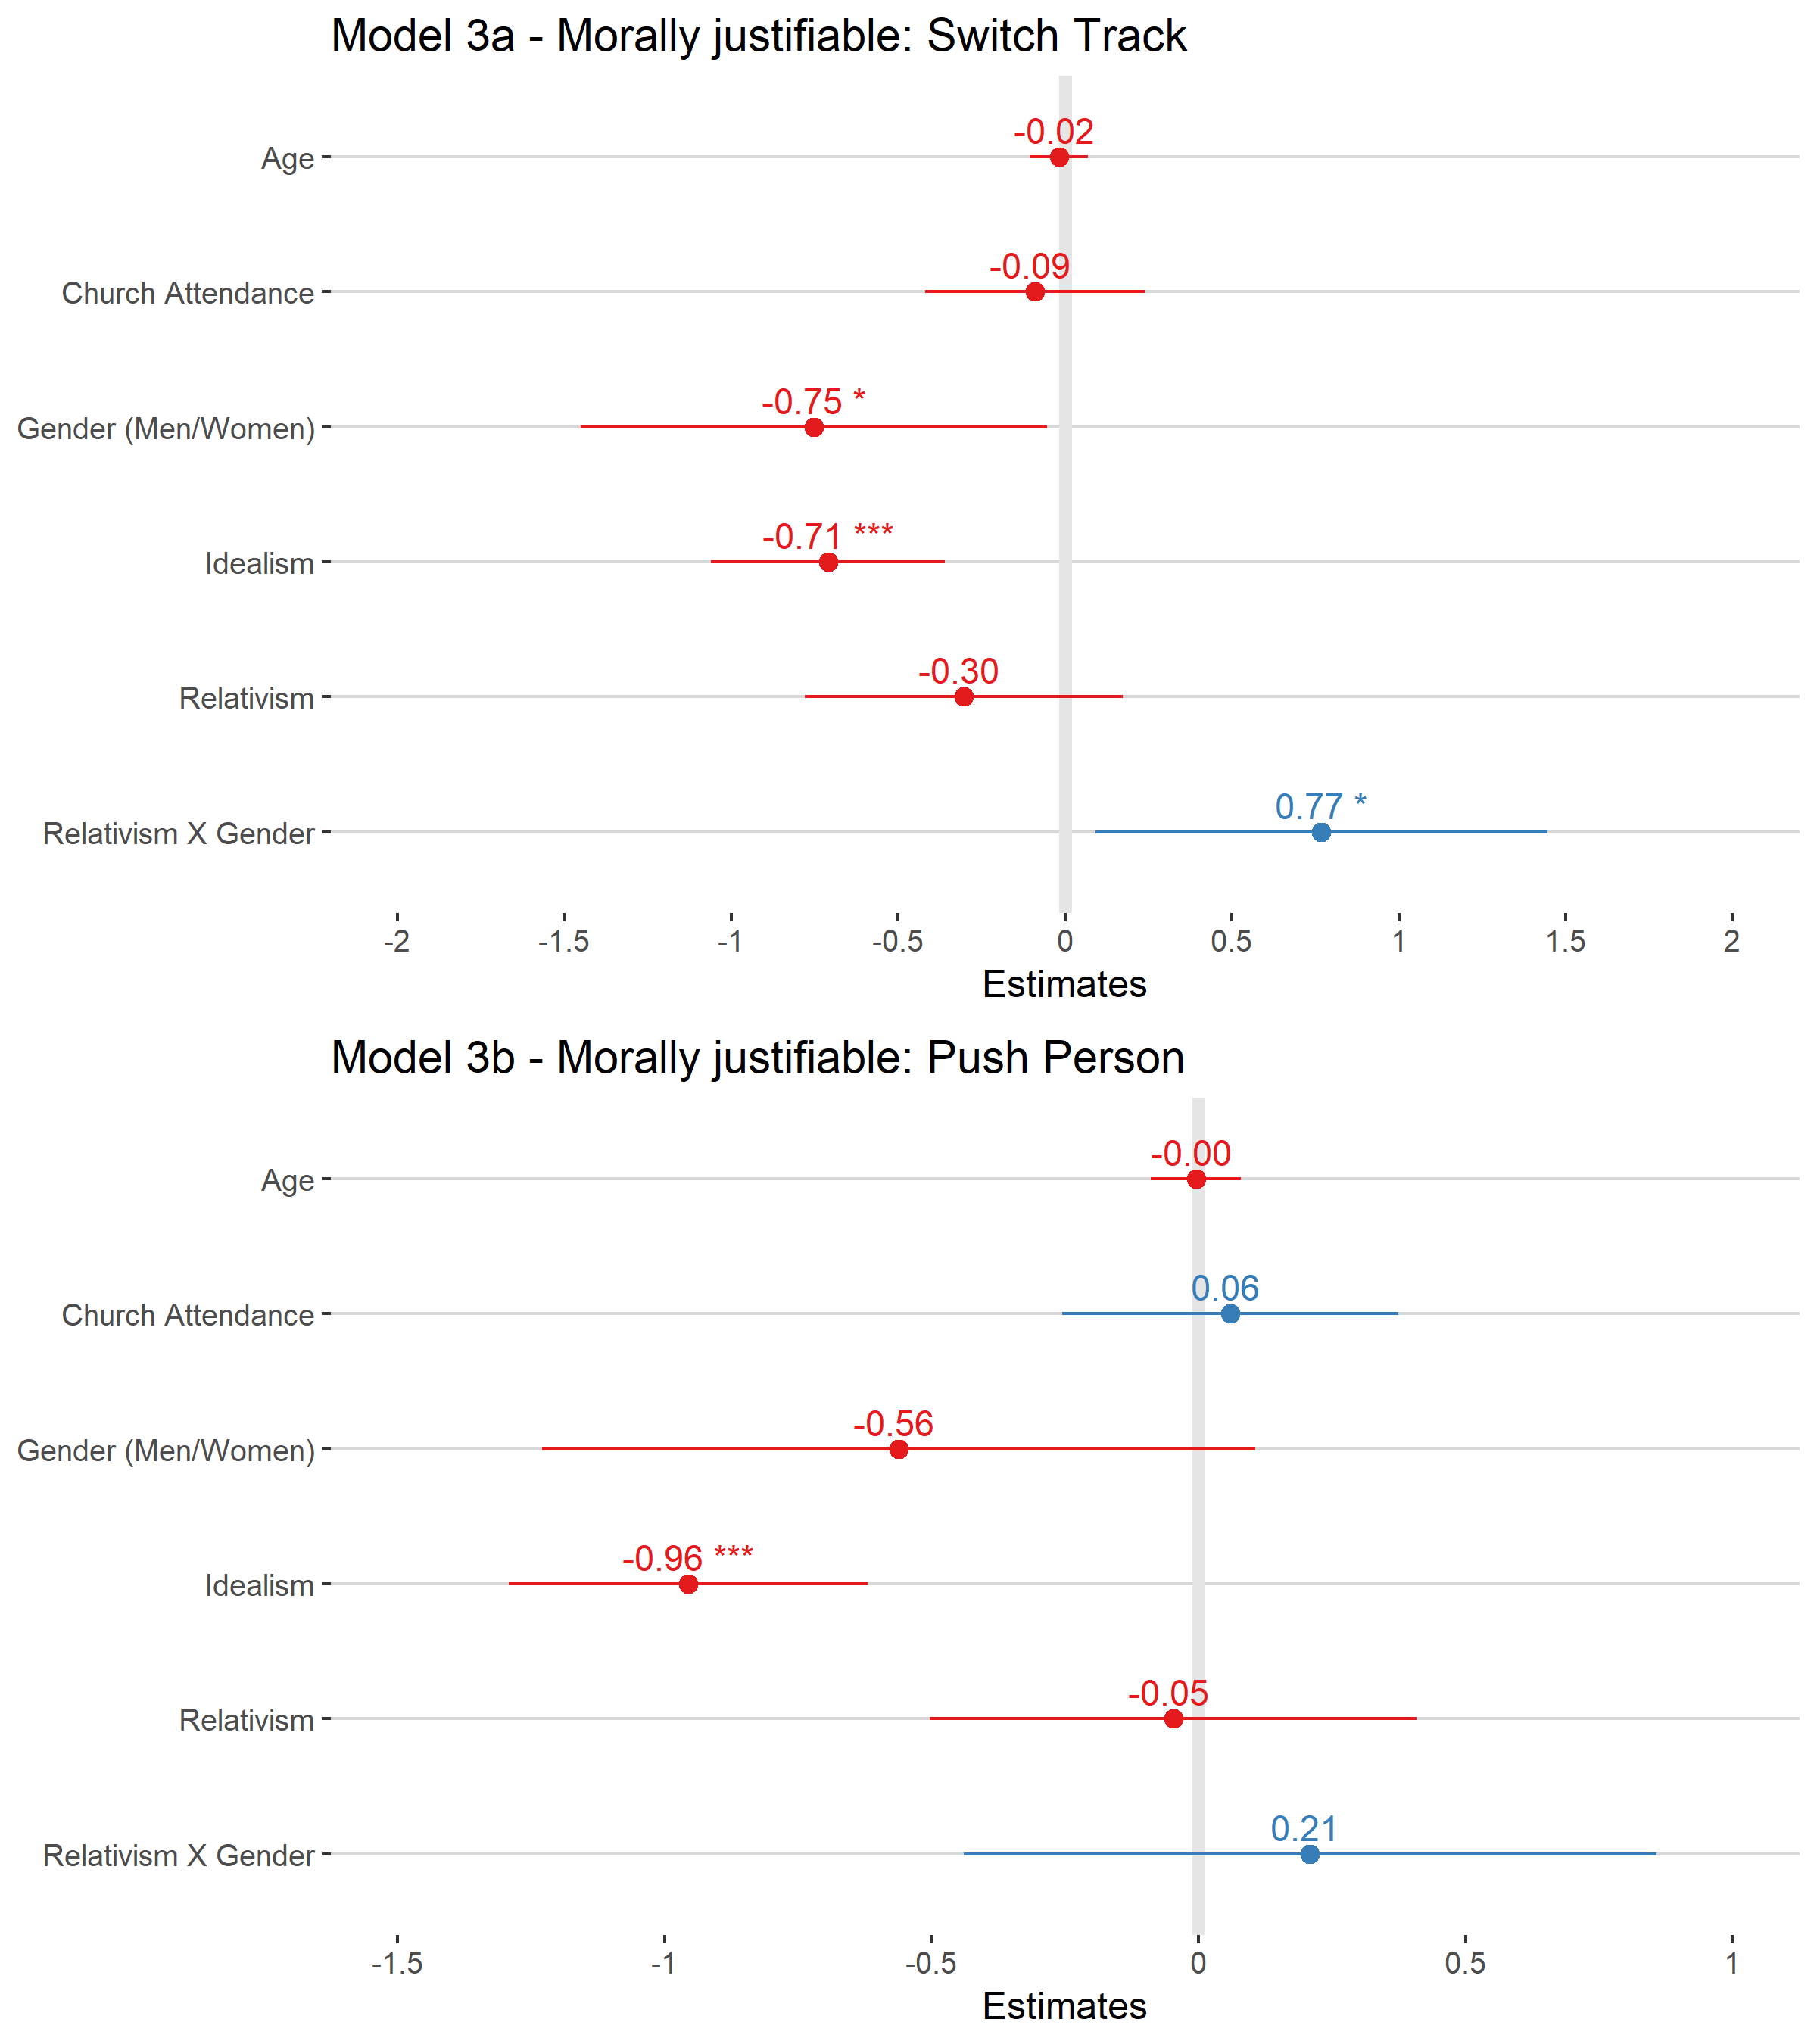
\includegraphics[width=\textwidth]{images/reg3_c1_relativism}
    \flushright
{\scriptsize $^{***}p<0.001$, $^{**}p<0.01$, $^*p<0.05$. N = 278. Unstandardized regression coefficients. 90\% confidence intervals are shown. \\ Own calculations based on data from Online-Survey Experiment.\par}
\end{figure}

In Models 3a and 3b, an interaction effect with the treatment and
idealism is estimated to test hypothesis H2a and H2b ( Compared to the
control group, information and discussion treatment, respectively,
strengthen the effect of idealism on decision to not switch/push) . Plot
xx and XX show the marginal effects for the interactions, respectively.
The reported results do not point in the direction assumed in the
hypotheses. XXX Hier wären die Interaction plots toll.XXXX

\begin{figure}[!h]
    \caption{Models 3 - Relativism Interaction Plots}
    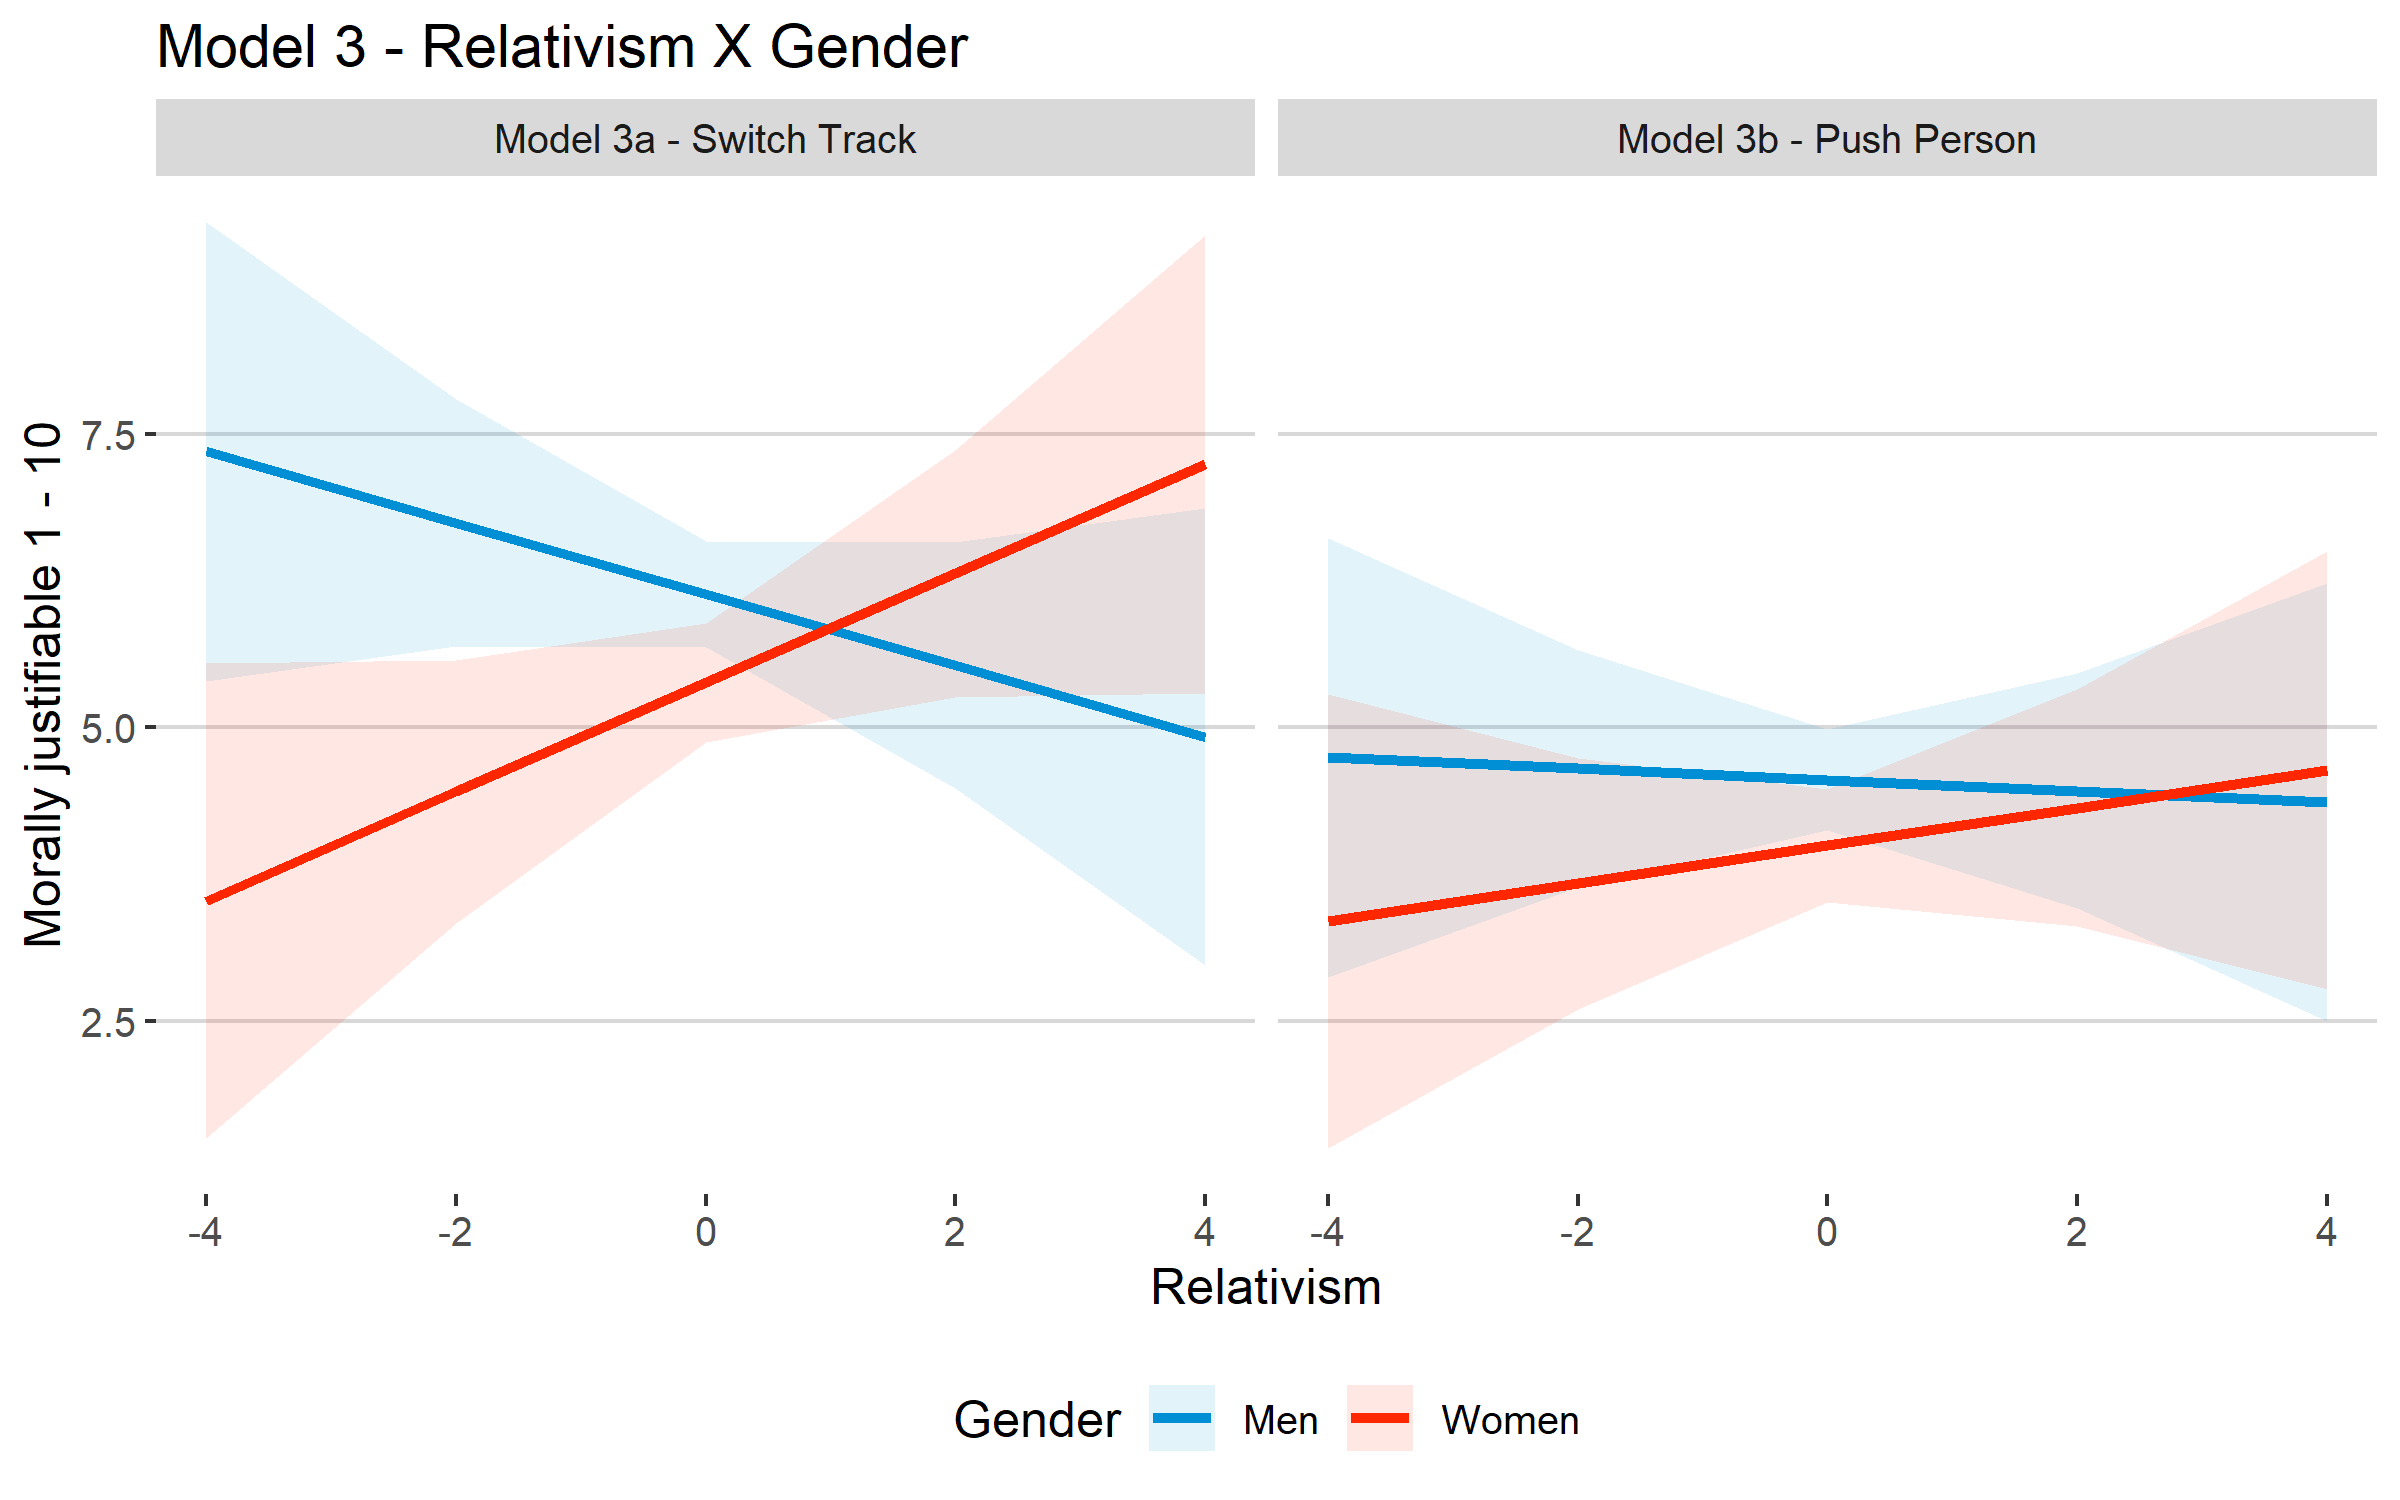
\includegraphics[width=\textwidth]{images/reg3_c2_relativism}
    \flushright
{\scriptsize N = 278. 90\% confidence intervals are shown. \\ Own calculations based on data from Online-Survey Experiment.\par}
\end{figure}

Hier am Samstag weiter arbeiten

In Models 4a and 4b, an interaction effect with the treatment and
relativism is estimated. Plot xx and XX show the marginal effects for
the interactions, respectively. It appears that for relativism, there
is\ldots{} XXX Auch hier wären die Interaction plots toll.XXXX

\begin{figure}[!h]
    \caption{Models 4 - Opinion Change}
    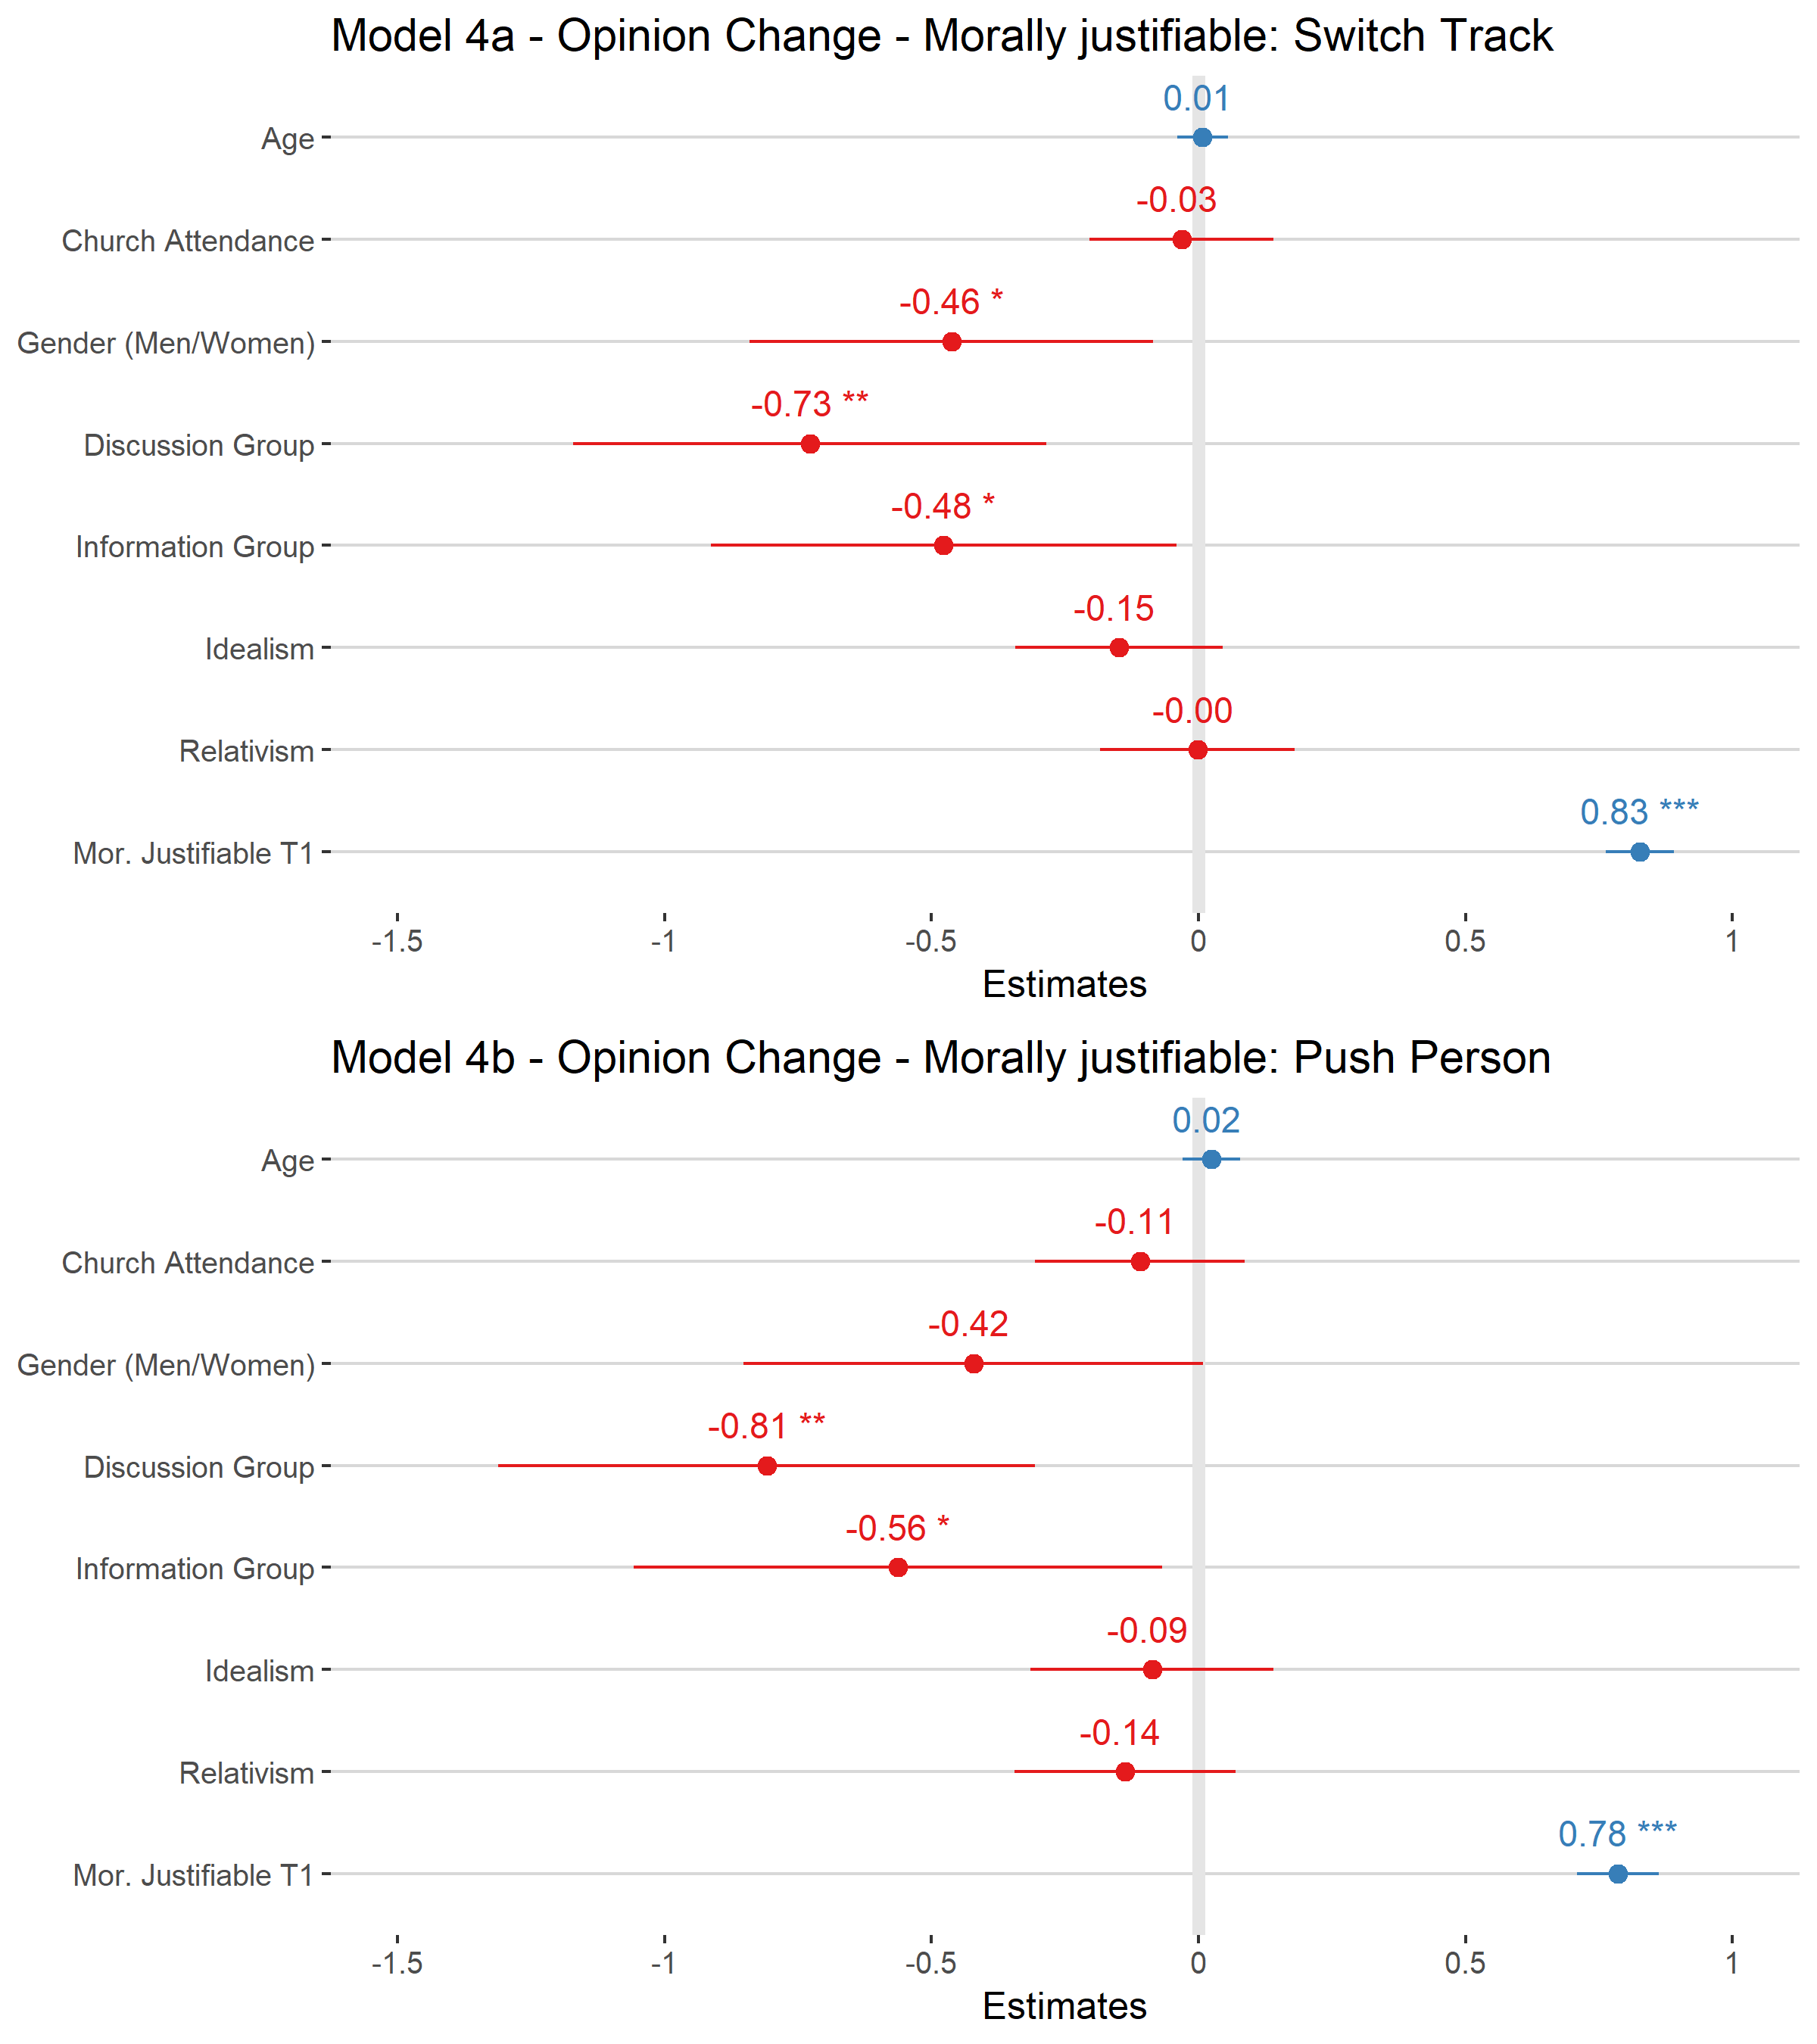
\includegraphics[width=\textwidth]{images/reg4_combined}
    \flushright
{\scriptsize $^{***}p<0.001$, $^{**}p<0.01$, $^*p<0.05$. N = 278. Unstandardized regression coefficients. 90\% confidence intervals are shown. \\ Own calculations based on data from Online-Survey Experiment.\par}
\end{figure}

Hier am Samstag weiter arbeiten H3a: In general, relativism has no
effect on the direction of opinion change. -\textgreater{} nicht ganz so
bestätigt, bisschen durcheinander die effekte, aber alle nicht
signifikant H3b: The more relativist an individual is, the more likely
it will switch/push after receiving discussion treatment.
-\textgreater{} effektrichtung stimmt, aber nicht signifikant und nicht
sehr starker effekt

\begin{figure}[!h]
    \caption{Models 5 - Idealism}
    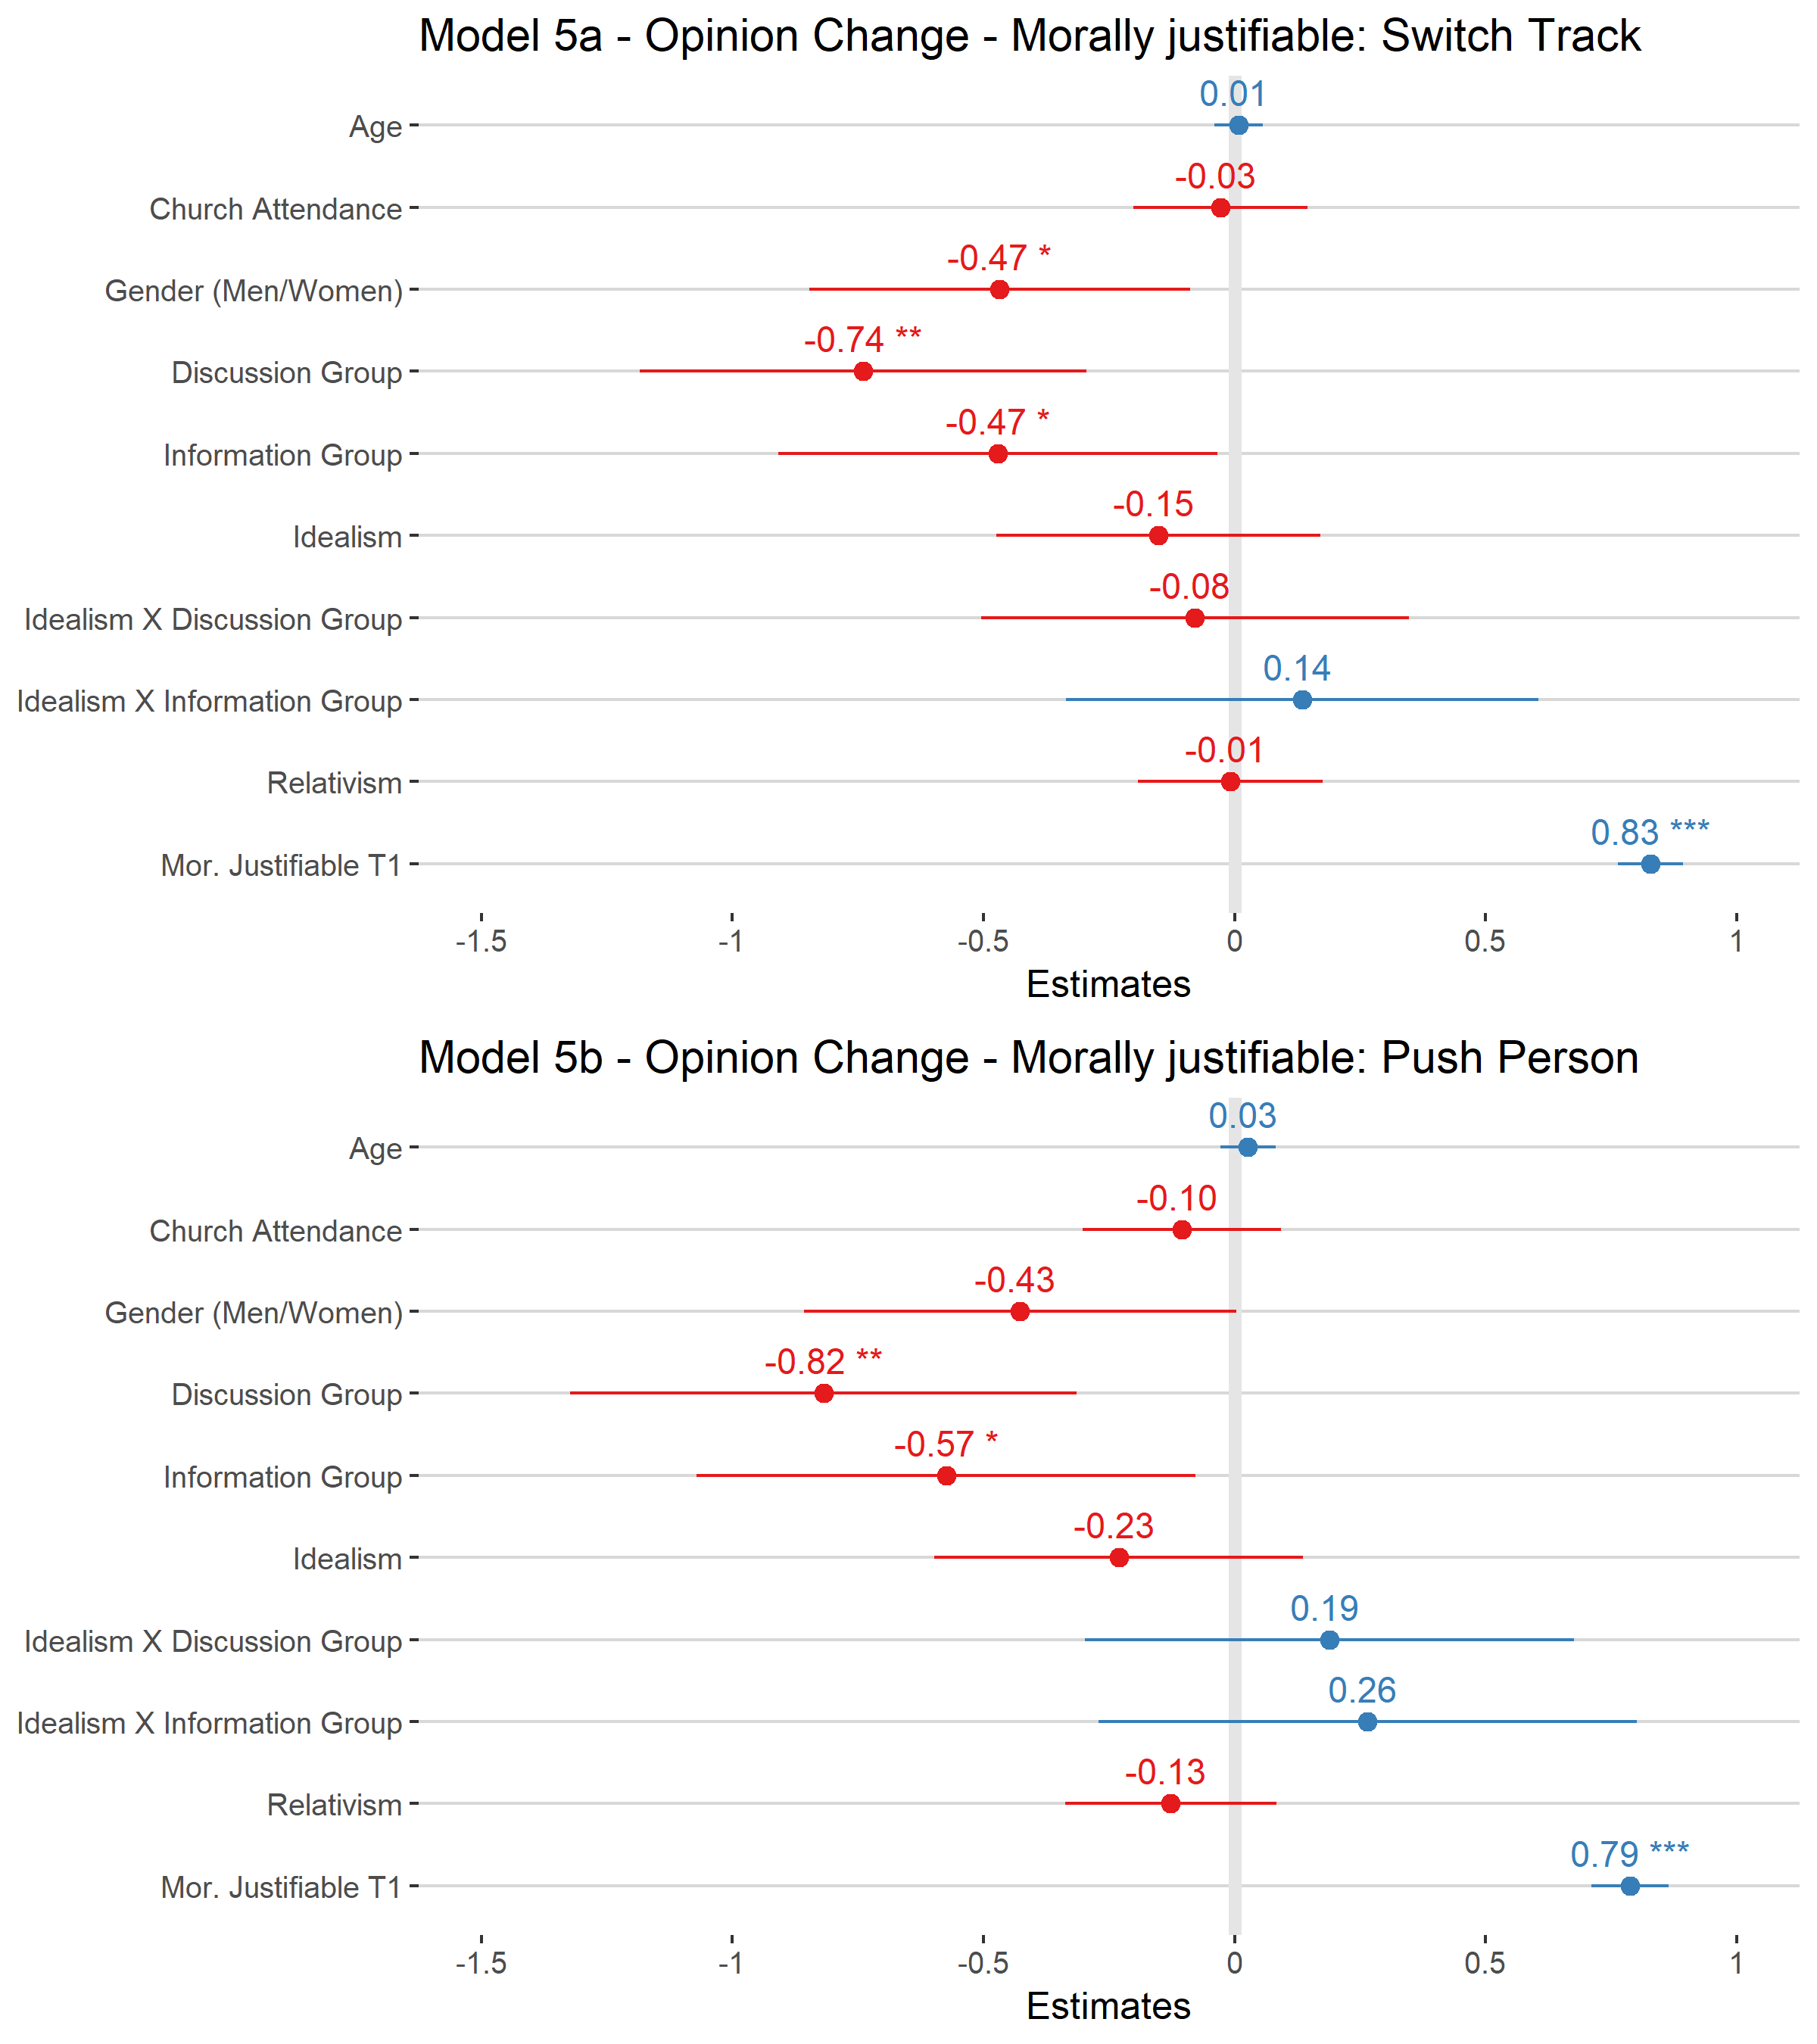
\includegraphics[width=\textwidth]{images/reg5_c1_idealism}
    \flushright
{\scriptsize $^{***}p<0.001$, $^{**}p<0.01$, $^*p<0.05$.  Unstandardized regression coefficients. 90\% confidence intervals are shown. \\ Own calculations based on data from Online-Survey Experiment.\par}
\end{figure}

Regarding the control variables for the dependent t1 variable, none of
them reaches statistical significance. In both models, a negative effect
is observed for gender. Women score lower on the dependent variables,
meaning that they are less inclined to switch/push. For both scenarios,
church attendance has a really small positive effect, while age has no
observable effect at all. Regarding the the control variables in the t2
models, gender has a negative and weakly significant effect, indicating
that opinion change was more negative for woman than man. The other
control variables have only weak and insignificant effects.

\begin{figure}[!h]
    \caption{Models 5 - Idealism Interaction Plots}
    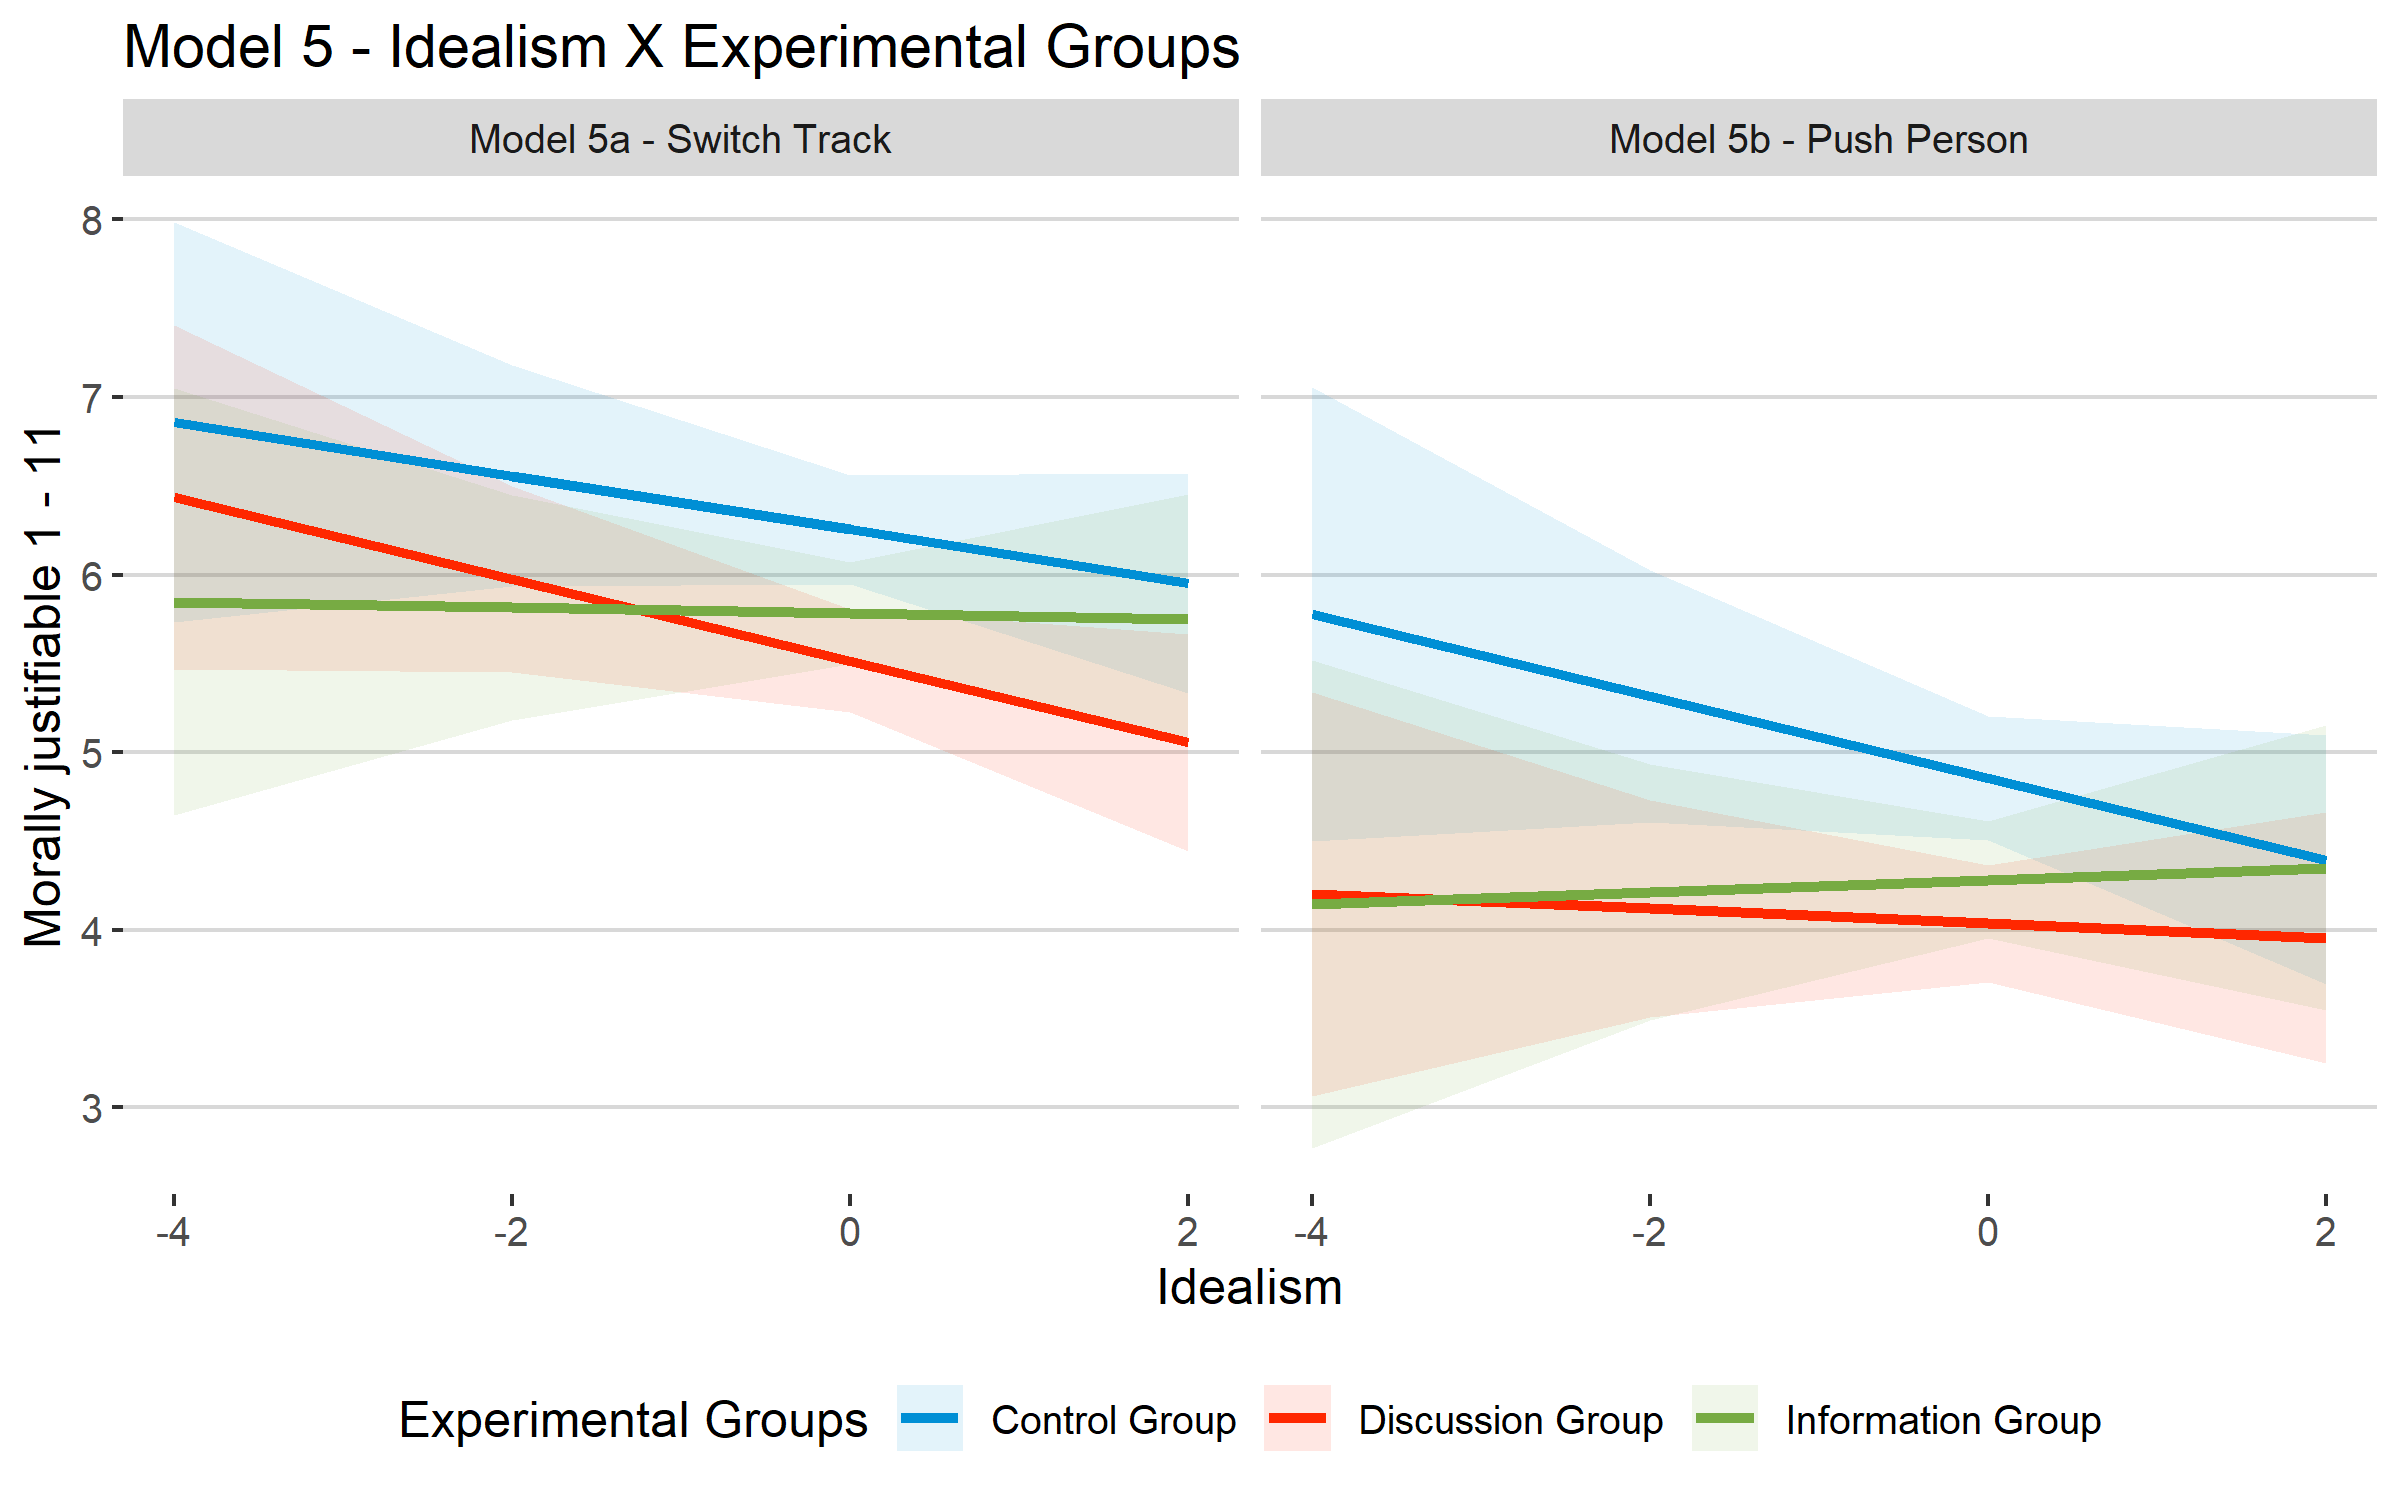
\includegraphics[width=\textwidth]{images/reg5_c2_idealism}
    \flushright
{\scriptsize N = 278. 90\% confidence intervals are shown. \\ Own calculations based on data from Online-Survey Experiment.\par}
\end{figure}

\begin{figure}[!h]
    \caption{Models 6 - Relativism}
    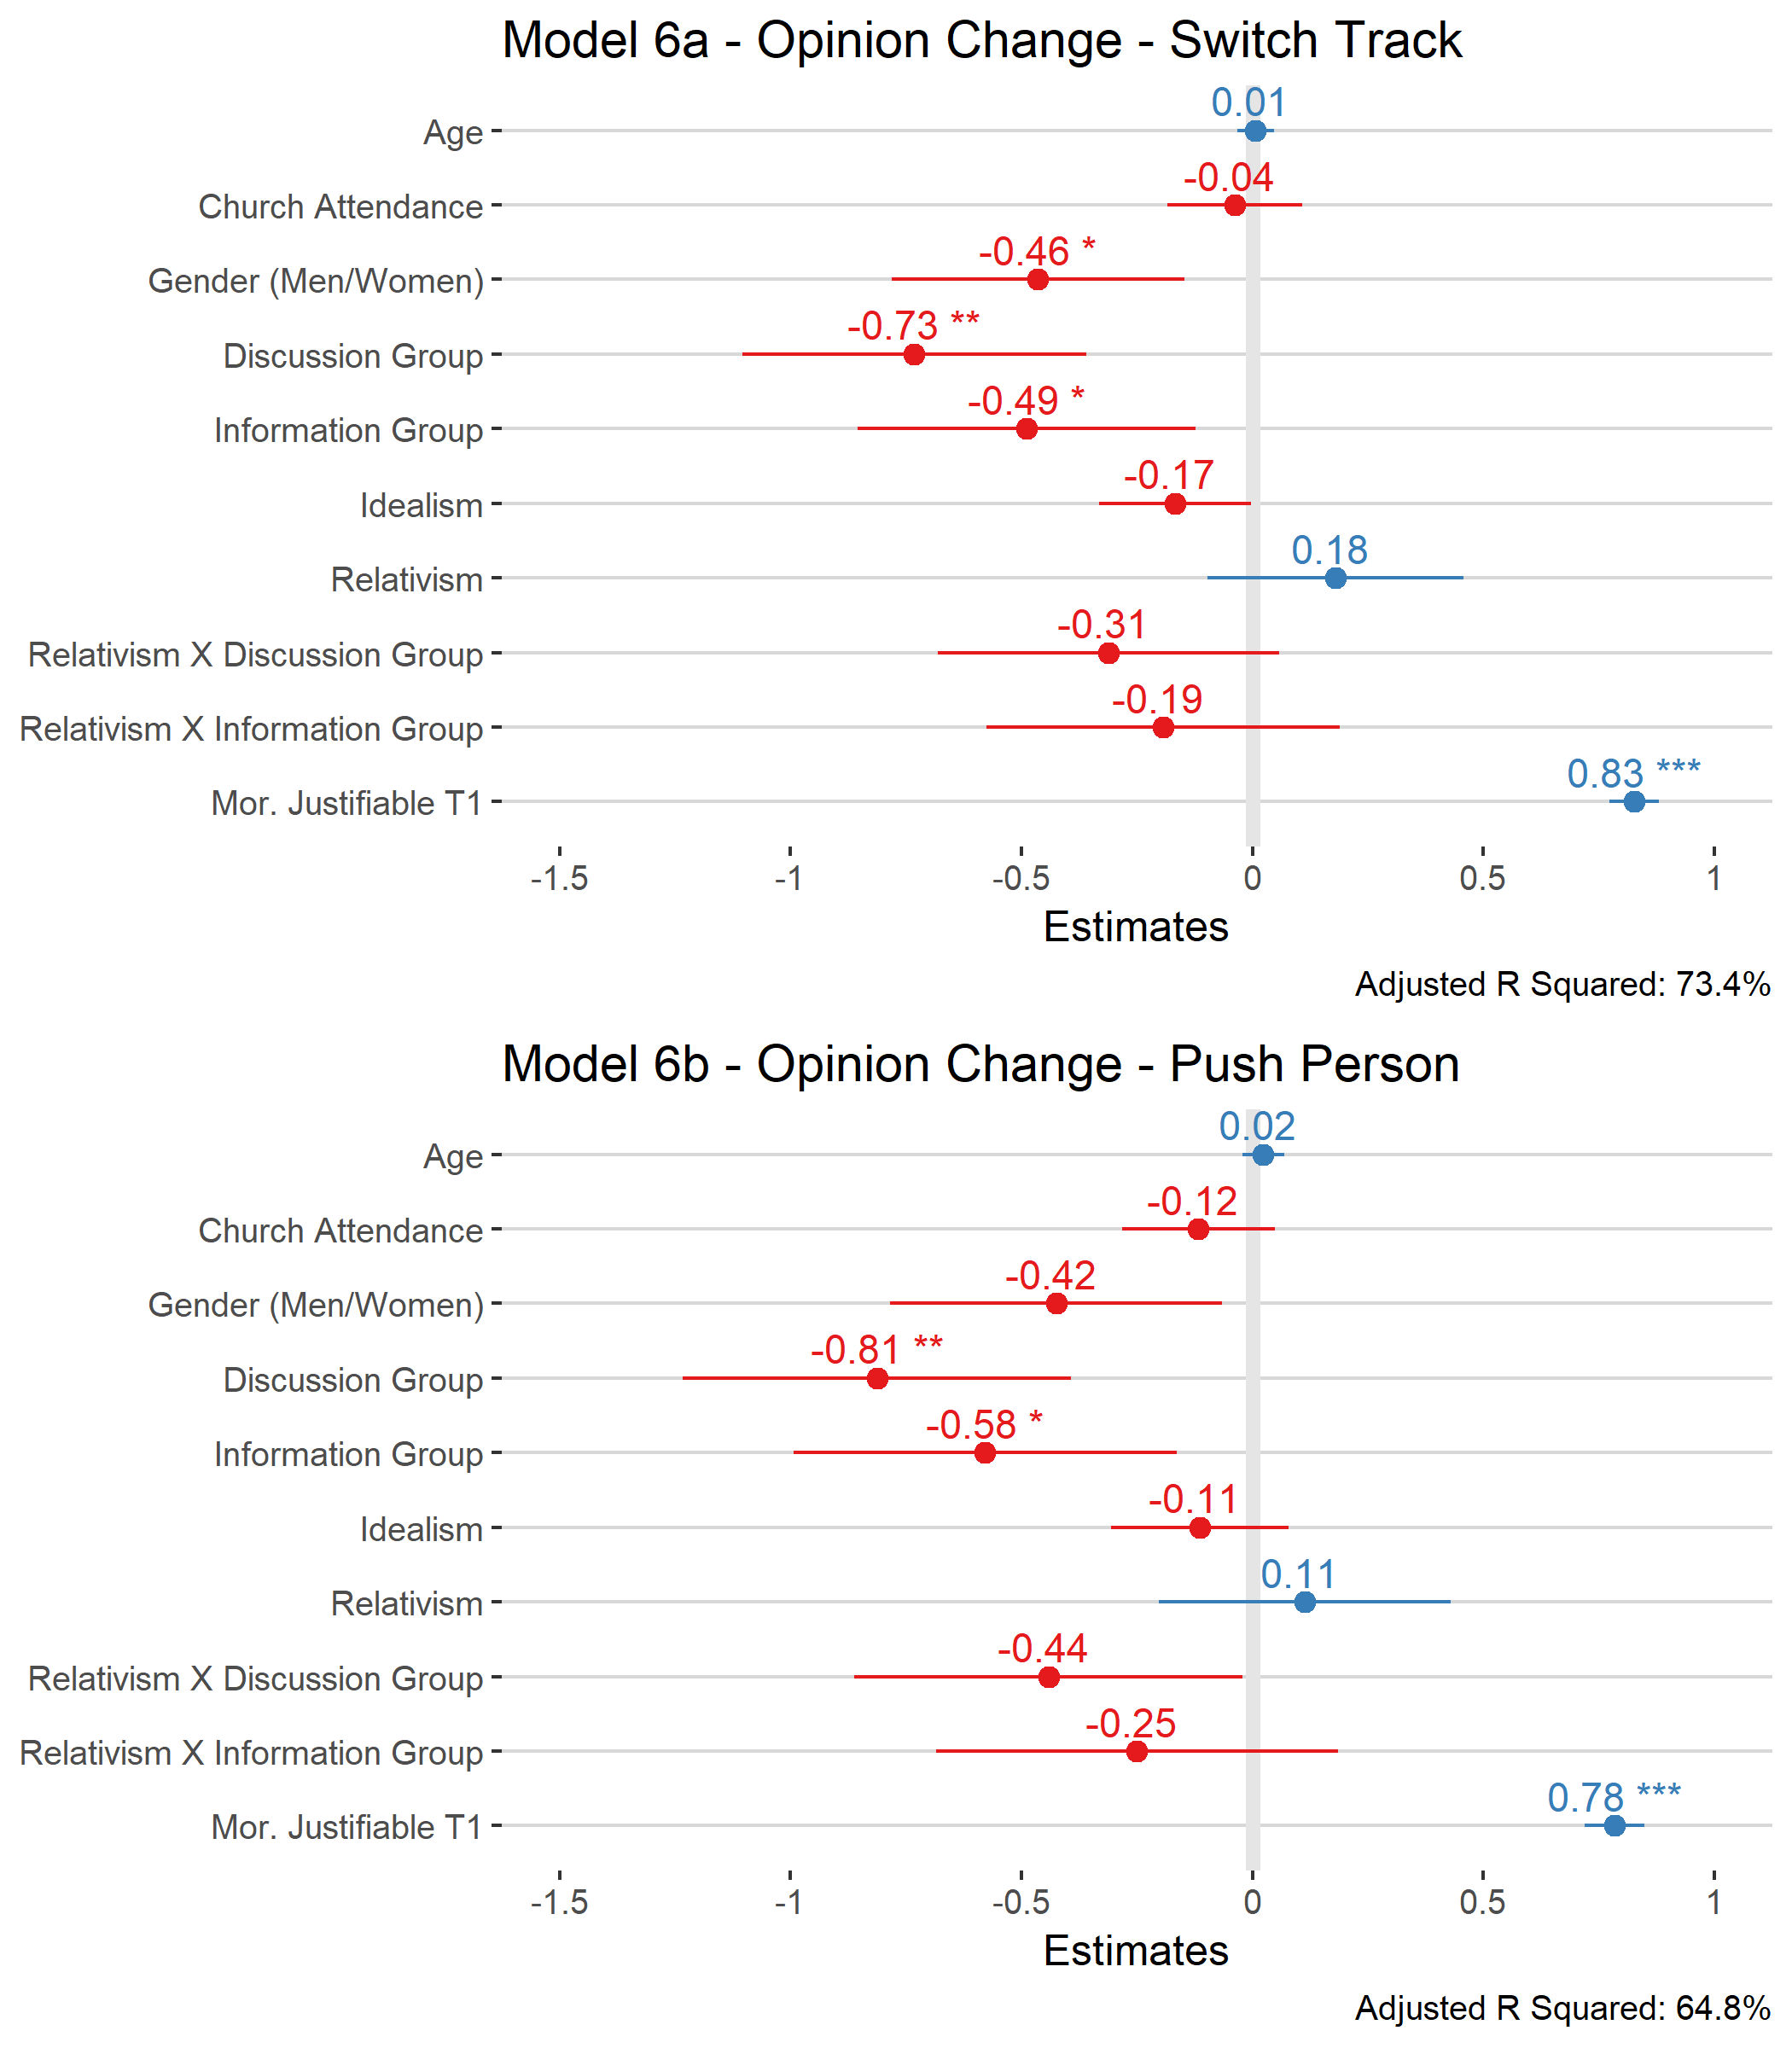
\includegraphics[width=\textwidth]{images/reg6_c1_relativism}
    \flushright
{\scriptsize $^{***}p<0.001$, $^{**}p<0.01$, $^*p<0.05$. N = 278. Unstandardized regression coefficients. 90\% confidence intervals are shown. \\ Own calculations based on data from Online-Survey Experiment.\par}
\end{figure}

\begin{figure}[!h]
    \caption{Models 6 - Relativism Interaction Plots}
    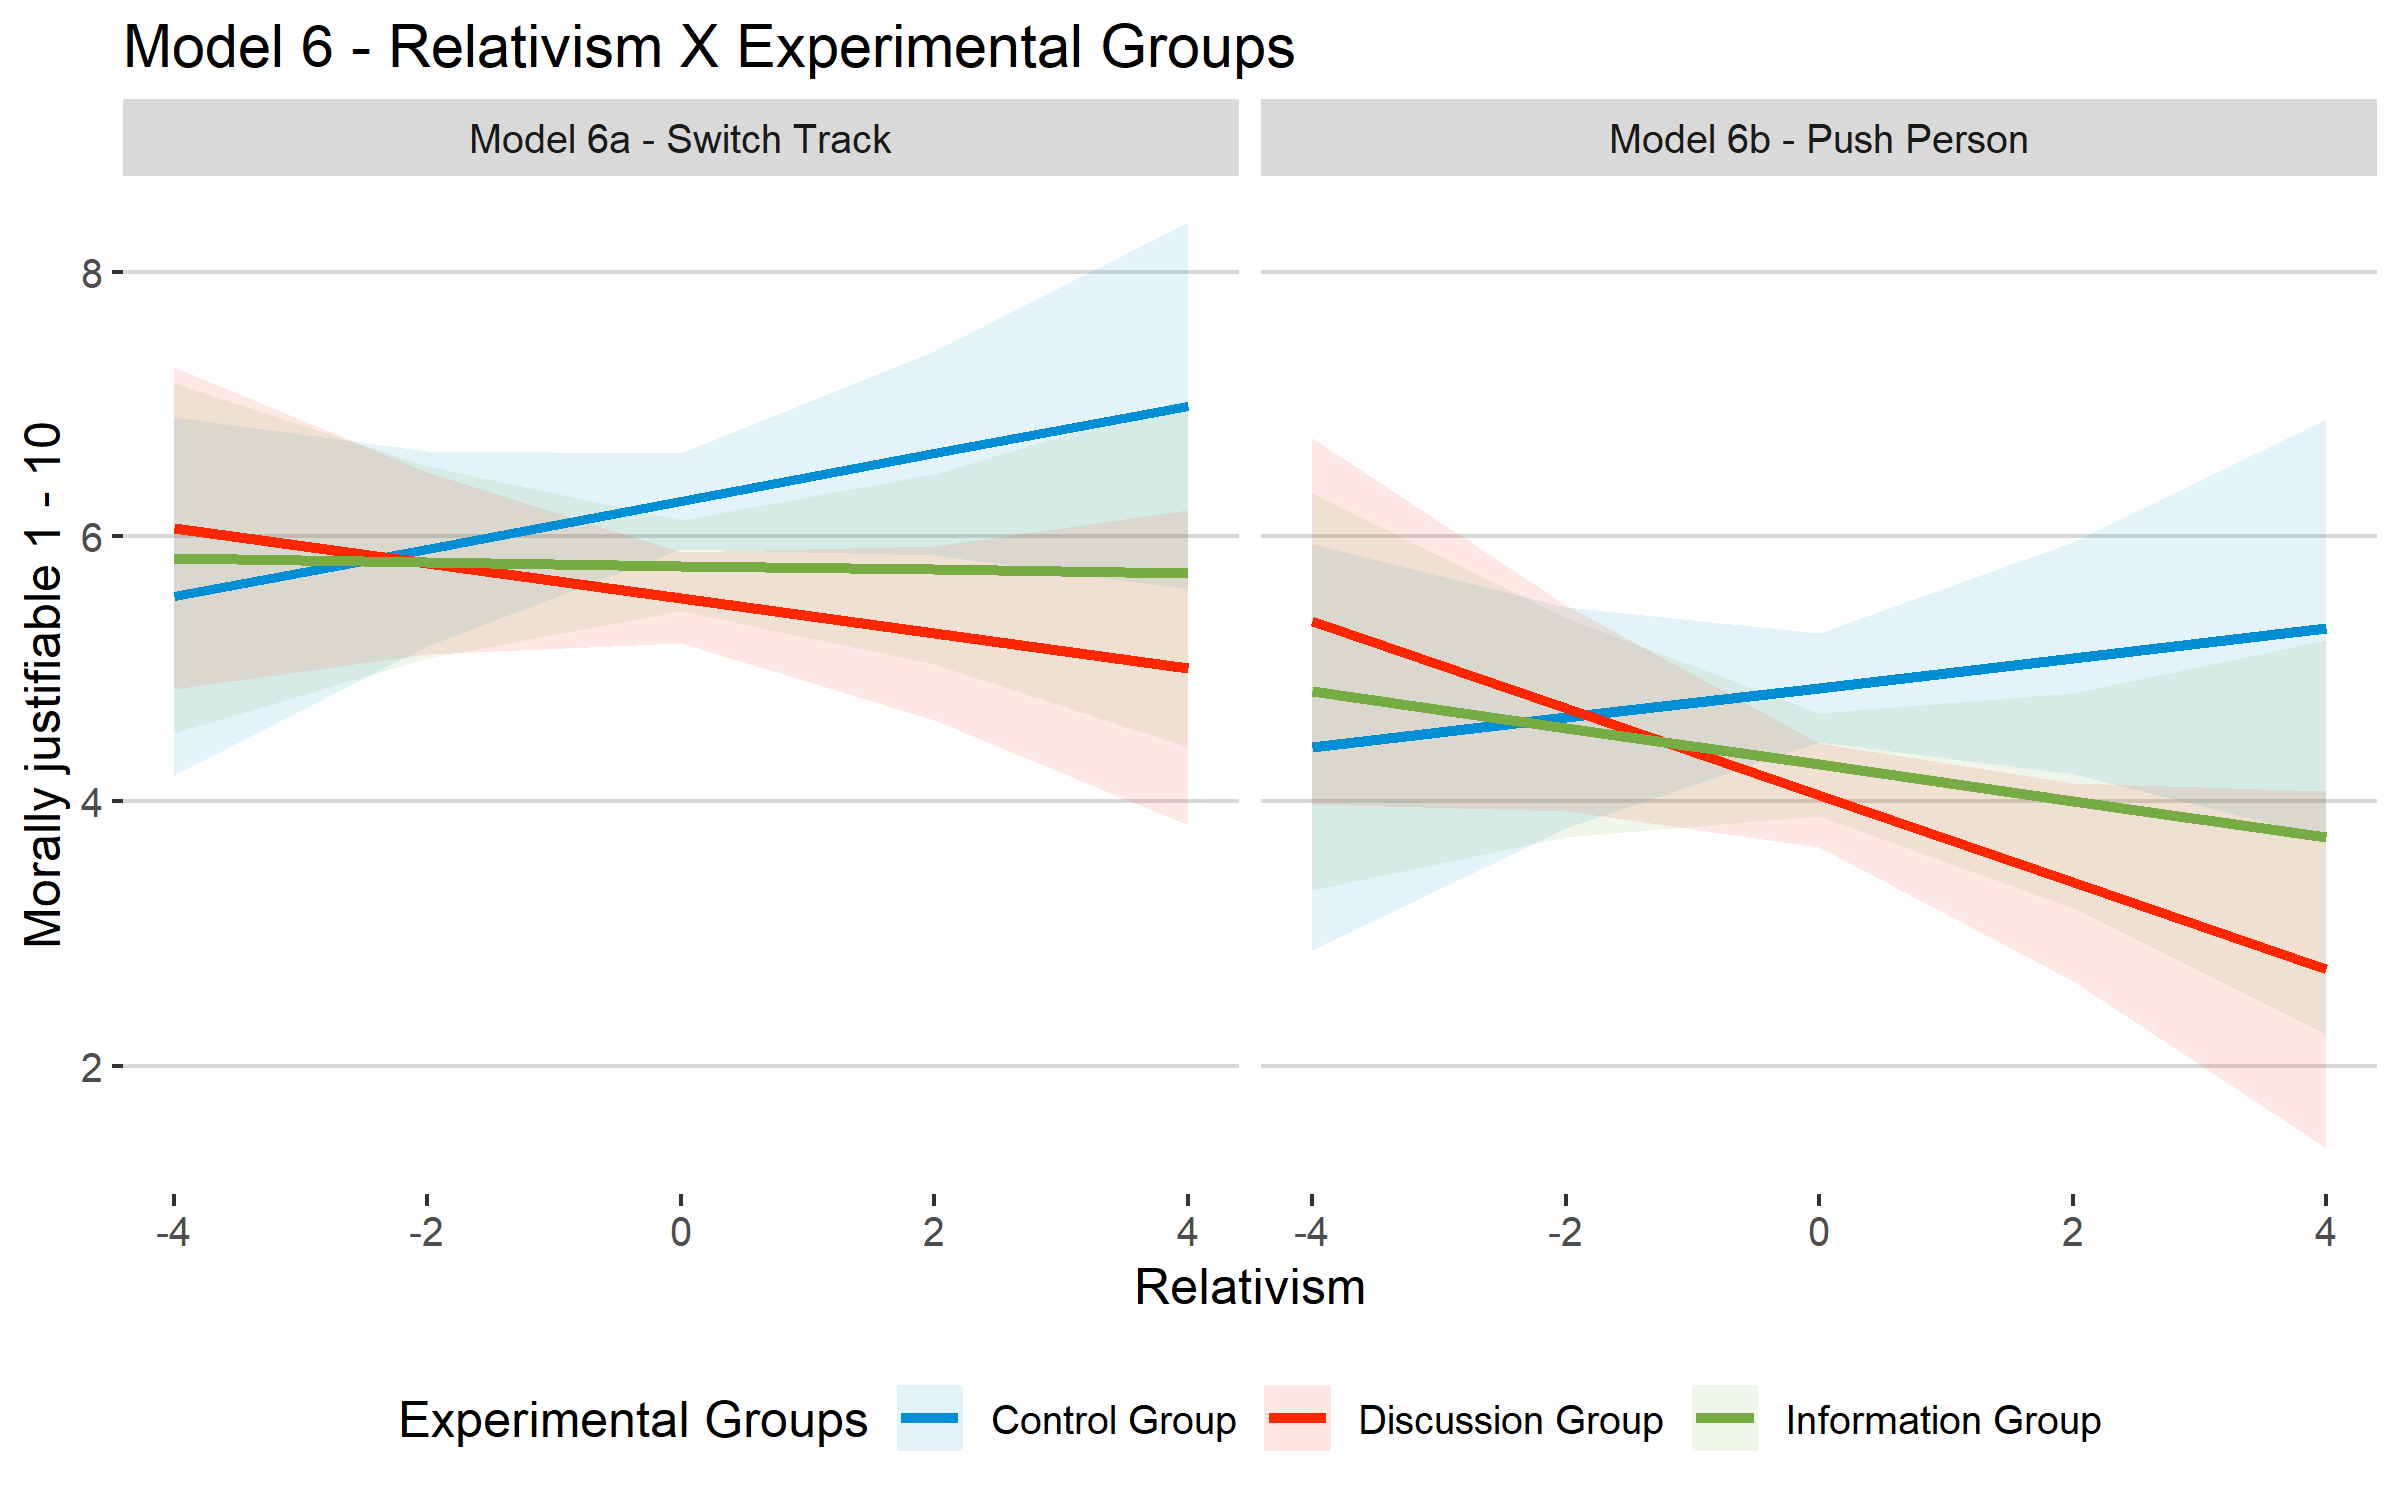
\includegraphics[width=\textwidth]{images/reg6_c2_relativism}
    \flushright
{\scriptsize N = 278. 90\% confidence intervals are shown. \\ Own calculations based on data from Online-Survey Experiment.\par}
\end{figure}

\newpage
\section{Conclusions} \label{conclusion}

Hypothesen die bestätigt wurden kurz erwähnen

Überlegen, warum Hypothesen ggf. nicht bestätigt wurden

Hier die Theorie zu Geschlecht einfügen? → yoh da haben ma doch wat.
Kann man zsm diskutieren

\setstretch{1}

\clearpage
\newpage

\hypertarget{references}{%
\section{References}\label{references}}

\setlength{\parindent}{-0.2in}
\setlength{\leftskip}{0.2in}
\setlength{\parskip}{8pt}

\noindent

\hypertarget{refs}{}
\leavevmode\hypertarget{ref-forsyth1980taxonomy}{}%
\textbf{Forsyth, Donelson R} \textbf{1980}: A taxonomy of ethical
ideologies., \emph{Journal of Personality and Social psychology} 39, pp.
175.

\leavevmode\hypertarget{ref-strack2007erfahrung}{}%
\textbf{Strack, Micha \& Gennerich, Carsten} \textbf{2007}: Erfahrung
mit forsyths' ethic position questionnaire?(EPQ):
Bedeutungsunabhängigkeit von idealismus und realismus oder akquieszens
und biplorarität?,

\newpage
\section{Appendix}
%\thispagestyle{empty}
%\pagenumbering{Roman} 	% R XI and r xi
%\addcontentsline{toc}{section}{Appendix}

%%% table settings
\setcounter{table}{0}
\renewcommand{\thetable}{A\arabic{table}}

\setcounter{figure}{0}
\renewcommand{\thefigure}{A\arabic{figure}}


% \setcounter{table}{1}
% \renewcommand{\thetable}{B\arabic{table}}
% \setcounter{figure}{1}
% \renewcommand{\thefigure}{B\arabic{figure}}


%---------------------------------------------------------------------------%
% Eigenständigkeiterklärung
%---------------------------------------------------------------------------%
\clearpage
\section*{Eigenständigkeitserklärung}
\vspace*{2cm}
\begin{center}
	\begin{minipage}[t]{0.8\textwidth}
		Hiermit versichern wir, dass wir die vorliegende Hausarbeit selbständig und nur mit den angegebenen Hilfsmitteln verfasst haben. Alle Passagen, die wir wörtlich als auch sinngemäß aus der Literatur oder aus anderen Quellen wie z. B. Internetseiten entnommen haben, sind deutlich als Zitat mit Angabe der Quelle kenntlich gemacht.
		
		\vspace*{60mm}
		Stuttgart, 30.09.2018
	\end{minipage}
\end{center}


\end{document}


\end{document}
